\chapter{Results and Discussion}
\label{chap:results}

\section{Chapter Overview}
This chapter presents the outcomes of the testing strategy defined in Chapter~\ref{ch:methodology}. 
Two distinct deployments were evaluated:
\begin{itemize}
  \item \textbf{Single VM (Quick Start):} Minimal environment on a resource-constrained laptop, including stress testing of SD-Core.
  \item \textbf{Full Aether (Lab PC):} Comprehensive environment (multiple UPFs, Aether ROC, network slicing) deployed in a lab setting, focusing on functional correctness at small scale.
\end{itemize}

\subsection{Recap of Test Scenarios}
As described in Section~\ref{sec:testing-strategy}, the core 5G scenarios include UE registration, PDU session establishment, AN (Access Network) release, UE-initiated service request, de-registration, and session release. 
In the single VM environment, we additionally perform load and stress tests. 
In the lab environment, we demonstrate advanced features (ROC, multiple UPFs, QoS) under relatively small-scale testing.

%===================================================

\section{Results: Single VM (Quick Start) Deployment}
The Quick Start testing was conducted within a \textbf{single VM}, simulating low to moderate UE loads. We detail each scenario’s measurements and discuss potential performance constraints. We first on the evaluation of a single UE deployment, then we consider deployment with multiple UE's.

\subsection{UE Registration}
\textbf{Objective \& Expectation}: Validate the AMF’s ability to authenticate and register a UE, with successful completion of the registration phase. 

\noindent \textbf{Observed Results}: 
\label{sec:results-discussion}
\begin{itemize}
    \item Our Python script indicates that for one or more UEs performing Registration, the \texttt{TotalRegTime[us]} metric remained within acceptable bounds.
    \item As load increased from 1 to N UEs, average registration time rose proportionally. No failures were observed.
\end{itemize}

\begin{figure}[H]
\centering
\caption{Registration Times (Seconds) for a Sample UE}
\label{fig:reg-times-sample-ue}
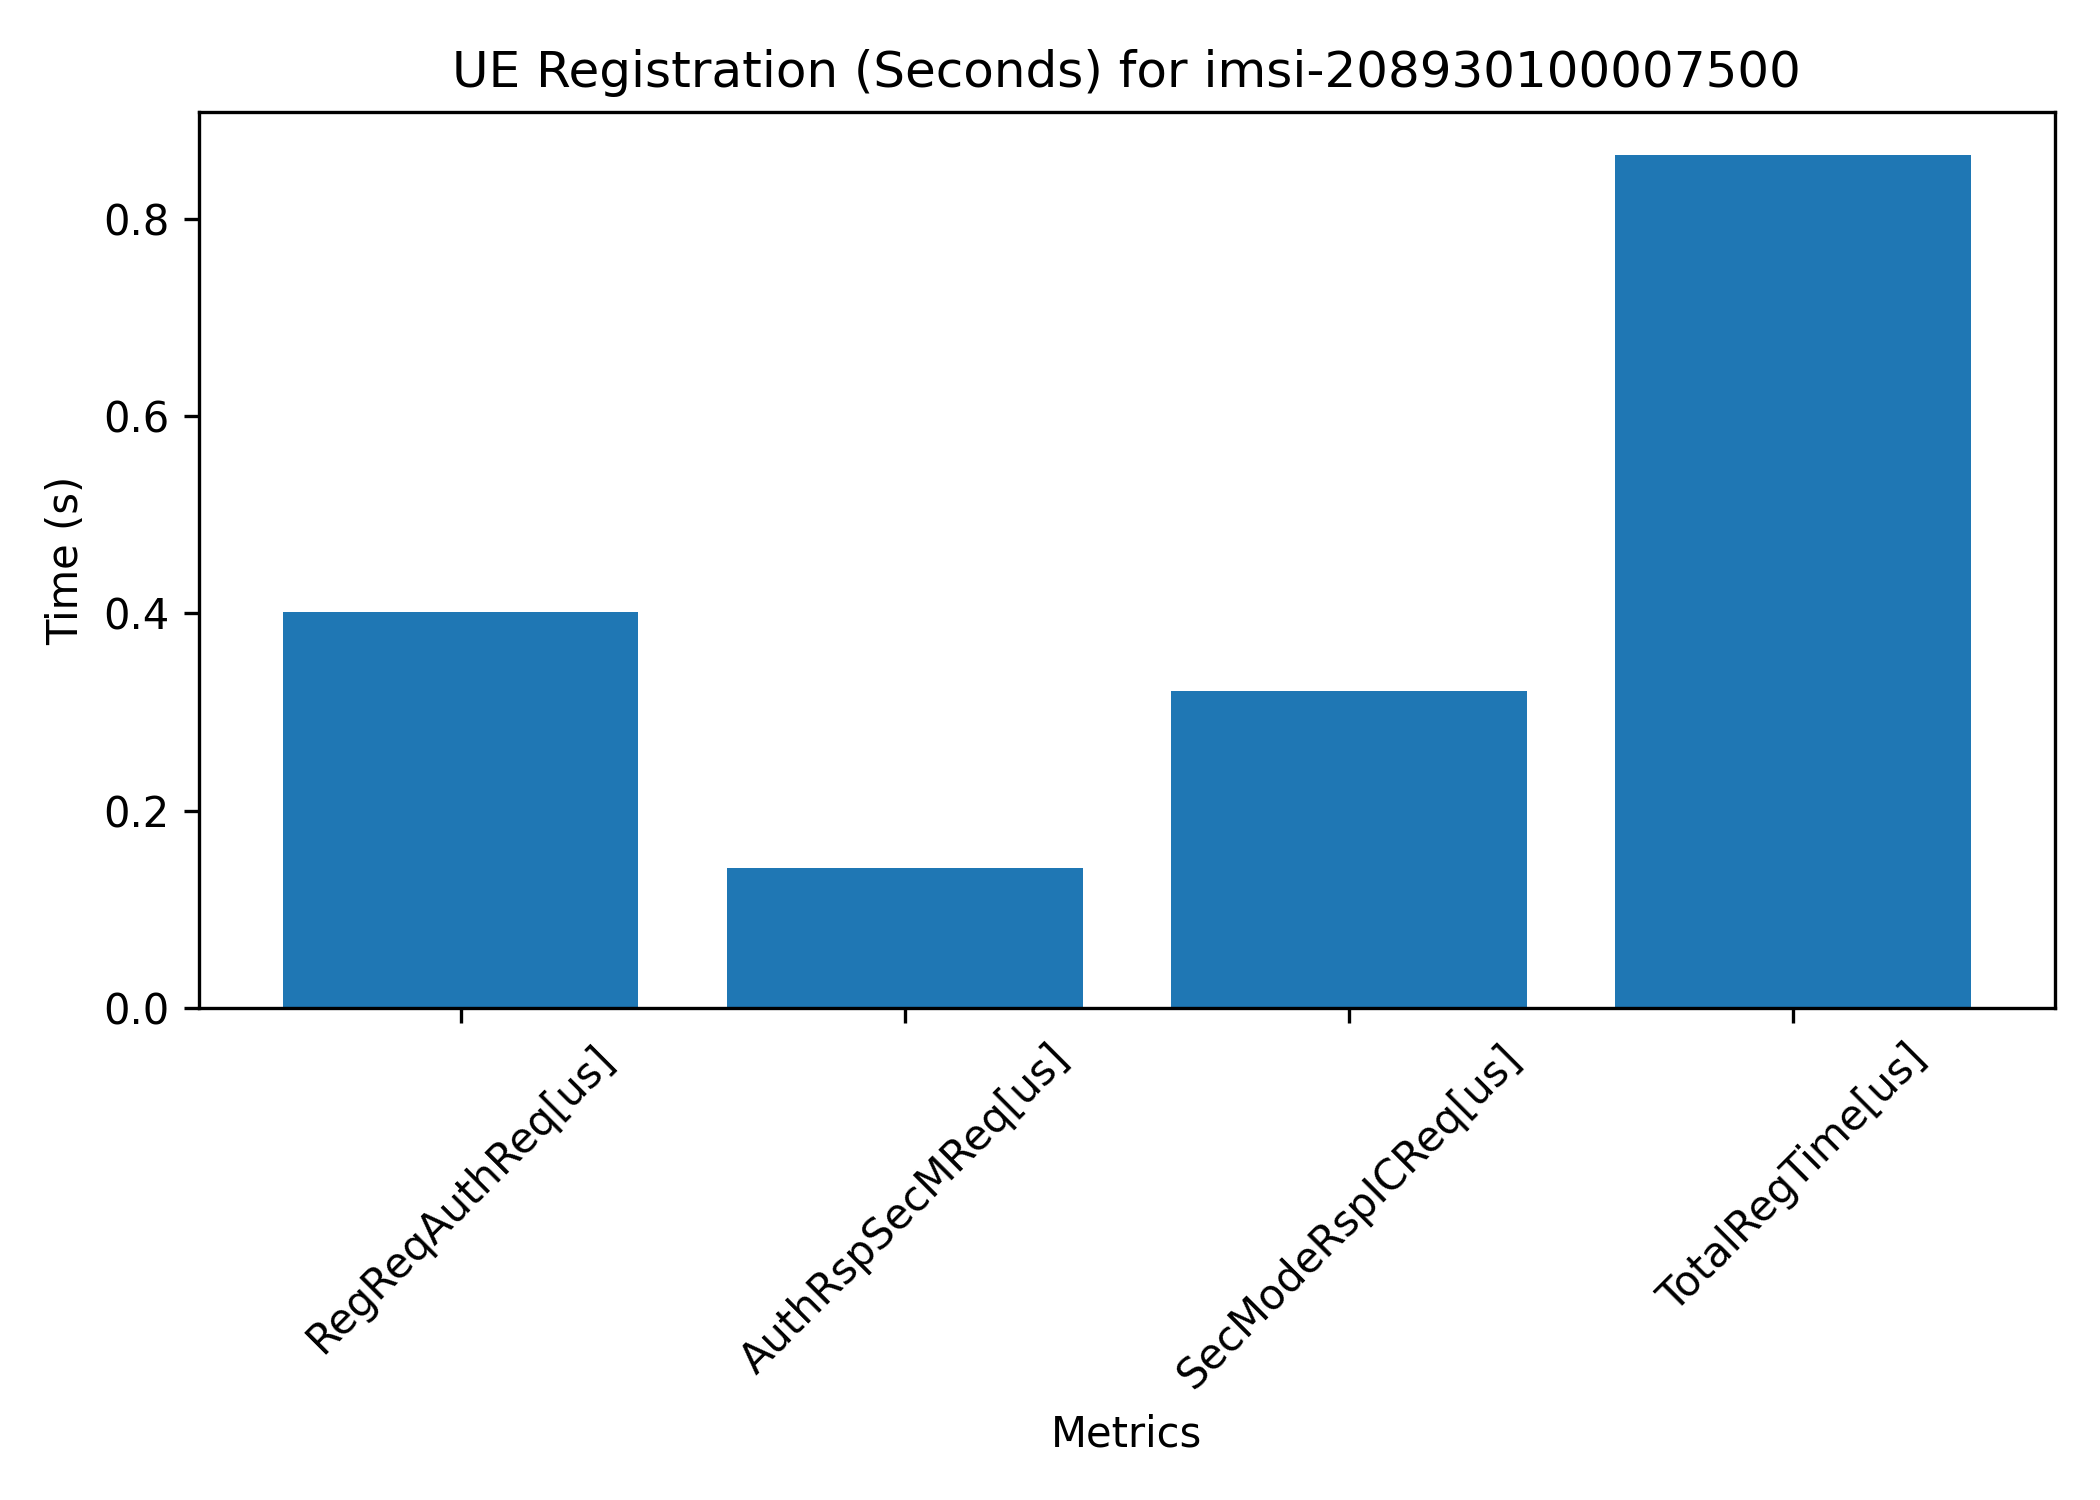
\includegraphics[width=0.6\textwidth]{Hassan_Thesis/images/Single Vm/Reults/1Uetest/UE_Registration_imsi-208930100007500.png}
\end{figure}

\paragraph{Discussion}\raggedright
The total time includes sub-phases (\texttt{RegReqAuthReq[us]}, \texttt{AuthRspSecMReq[us]}, \texttt{SecModeRspICReq[us]}). Minor increases in load caused modest latency growth, due to CPU scheduling in the single VM environment.

\subsection{UE-Initiated Session (PDU Session Establishment)}
\textbf{Objective \& Expectation}: Confirm successful establishment of a PDU session after registration, ensuring correct tunneling in the UPF.

\noindent \textbf{Observed Results}:
\begin{itemize}
    \item The metric \texttt{TotalPduEstTime[us]} was captured for each UE that initiated a session.
    \item Under higher loads, average session setup time increased, but no major failures were noted.
\end{itemize}

\begin{figure}[H]
\centering
\caption{PDU Session Establishment Times (Seconds) for a Sample UE}
\label{fig:pdu-sess-times-sample-ue}
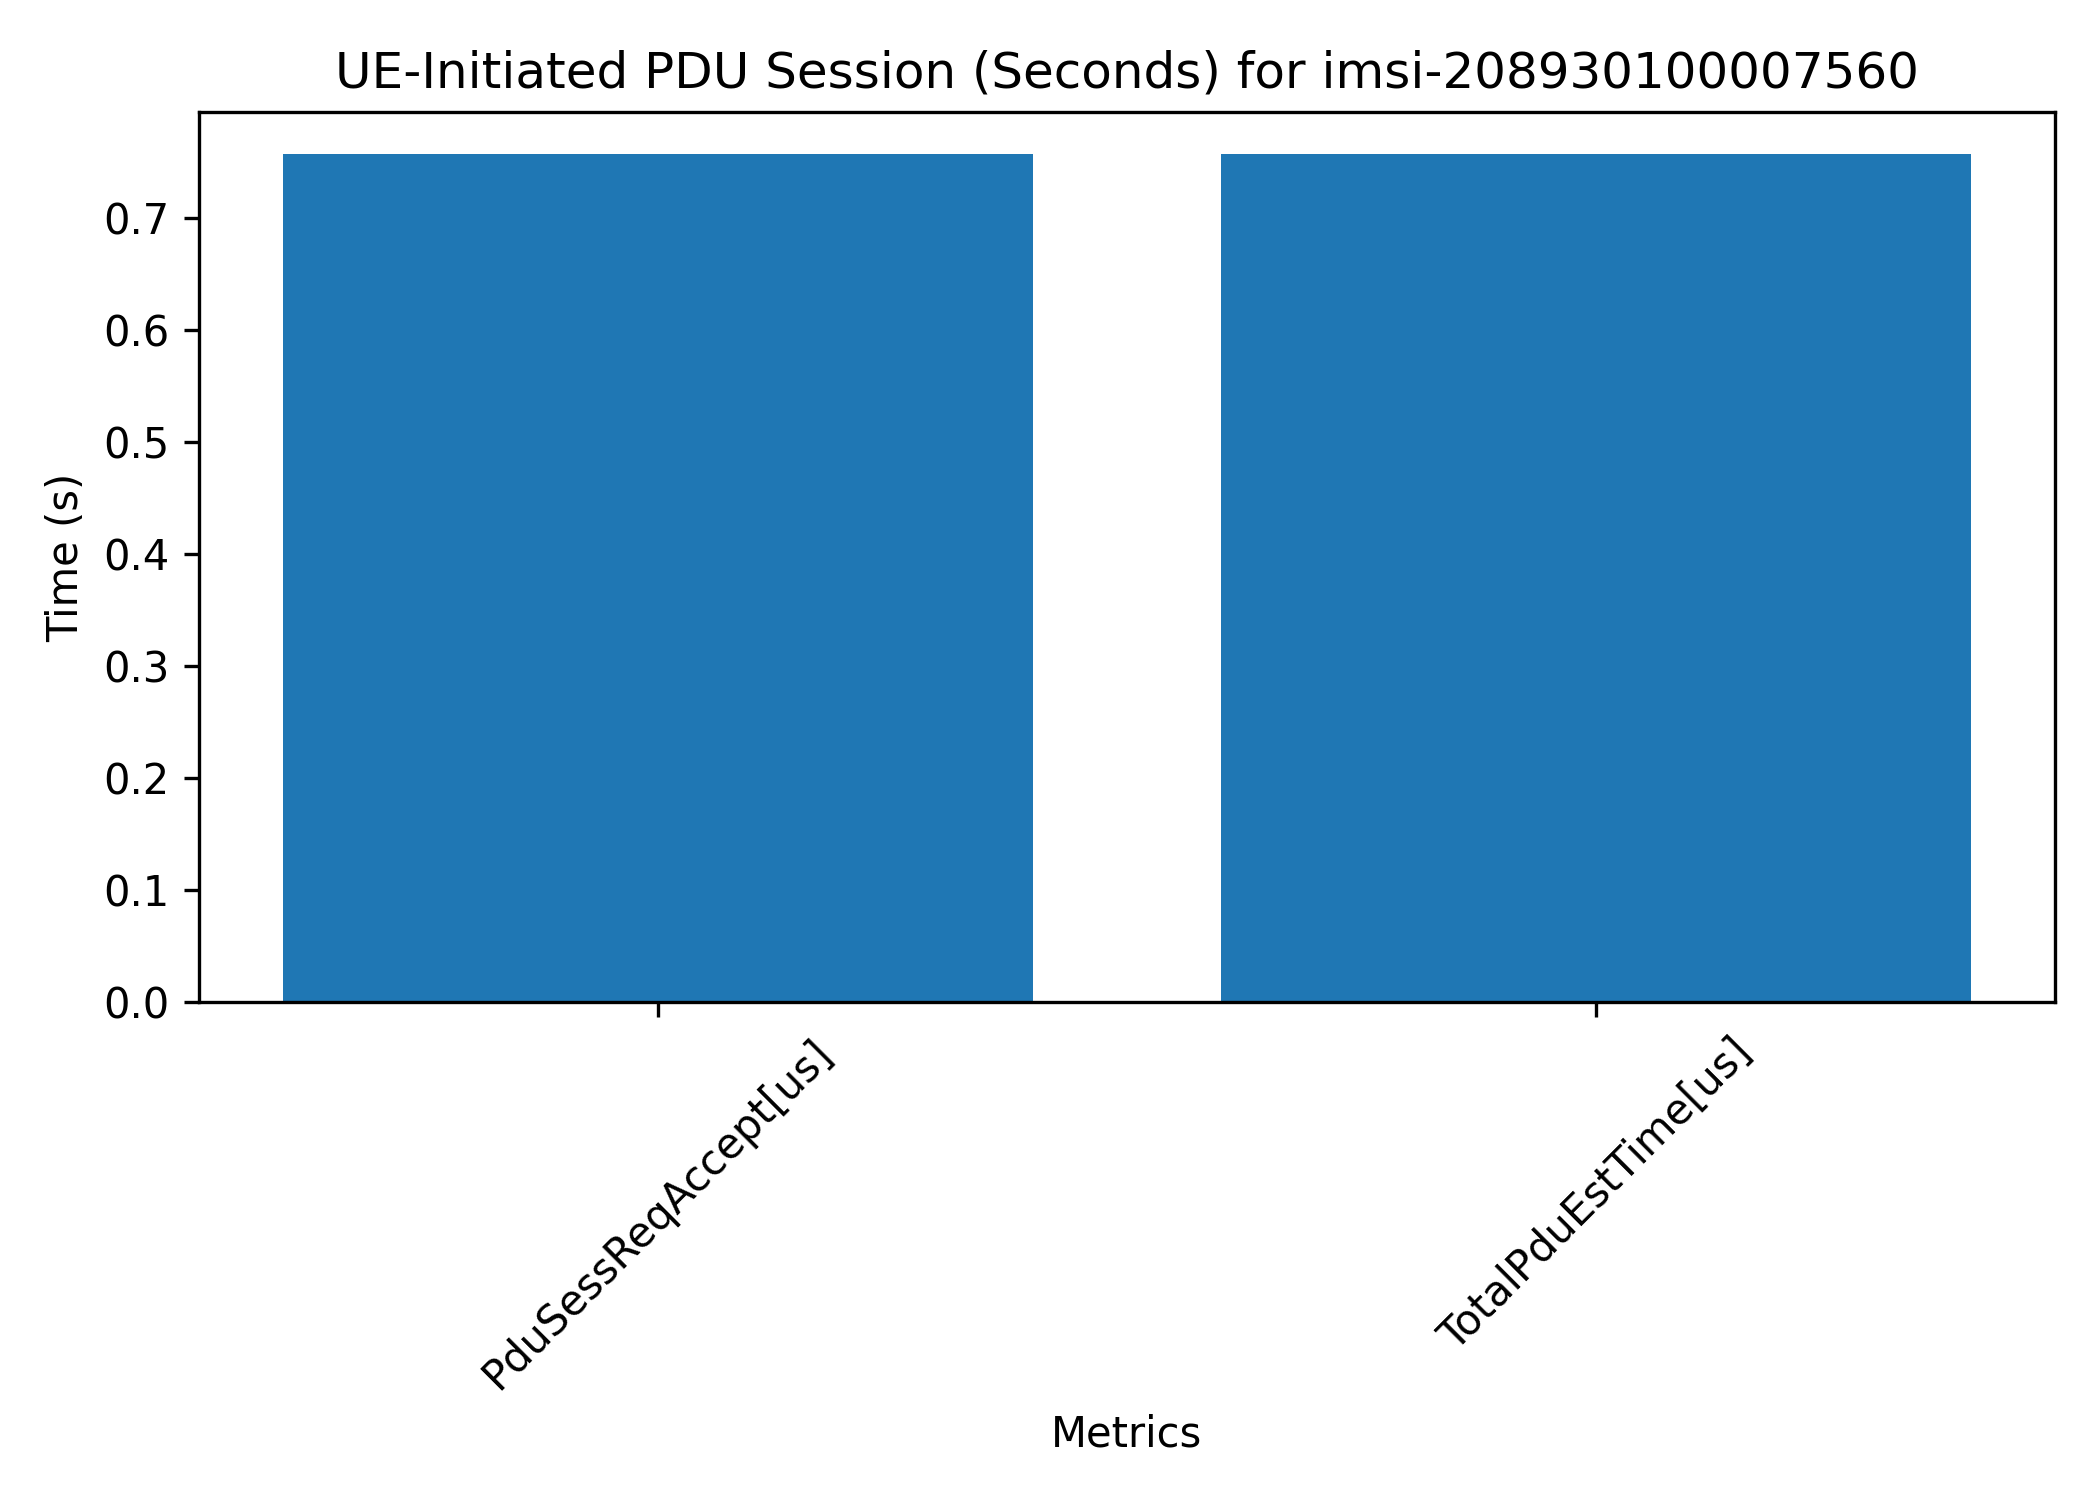
\includegraphics[width=0.6\textwidth]{Hassan_Thesis/images/Single Vm/Reults/1Uetest/UE-Initiated_PDU_Session_imsi-208930100007560.png}
\end{figure}

\paragraph{Discussion}
The sub-phase \texttt{PduSessReqAccept[us]} indicates the time from session request to acceptance. The total times remained within typical expected ranges for lab environments.

\subsection{Access Network (AN) Release}
\textbf{Objective \& Expectation}: Validate that AN resources are released efficiently when a UE moves out of coverage or transitions.

\noindent \textbf{Observed Results}:
\begin{itemize}
    \item \texttt{TotalCtxReleaseTime[us]} and \texttt{CtxRelReqCmdTime[us]} showed that resource cleanup occurred in a timely manner.
    \item No leftover or “stale” radio contexts were detected.
\end{itemize}

\begin{figure}[H]
\centering
\caption{Context Release Times (Seconds) for a Sample UE}
\label{fig:ctx-rel-times-sample-ue}
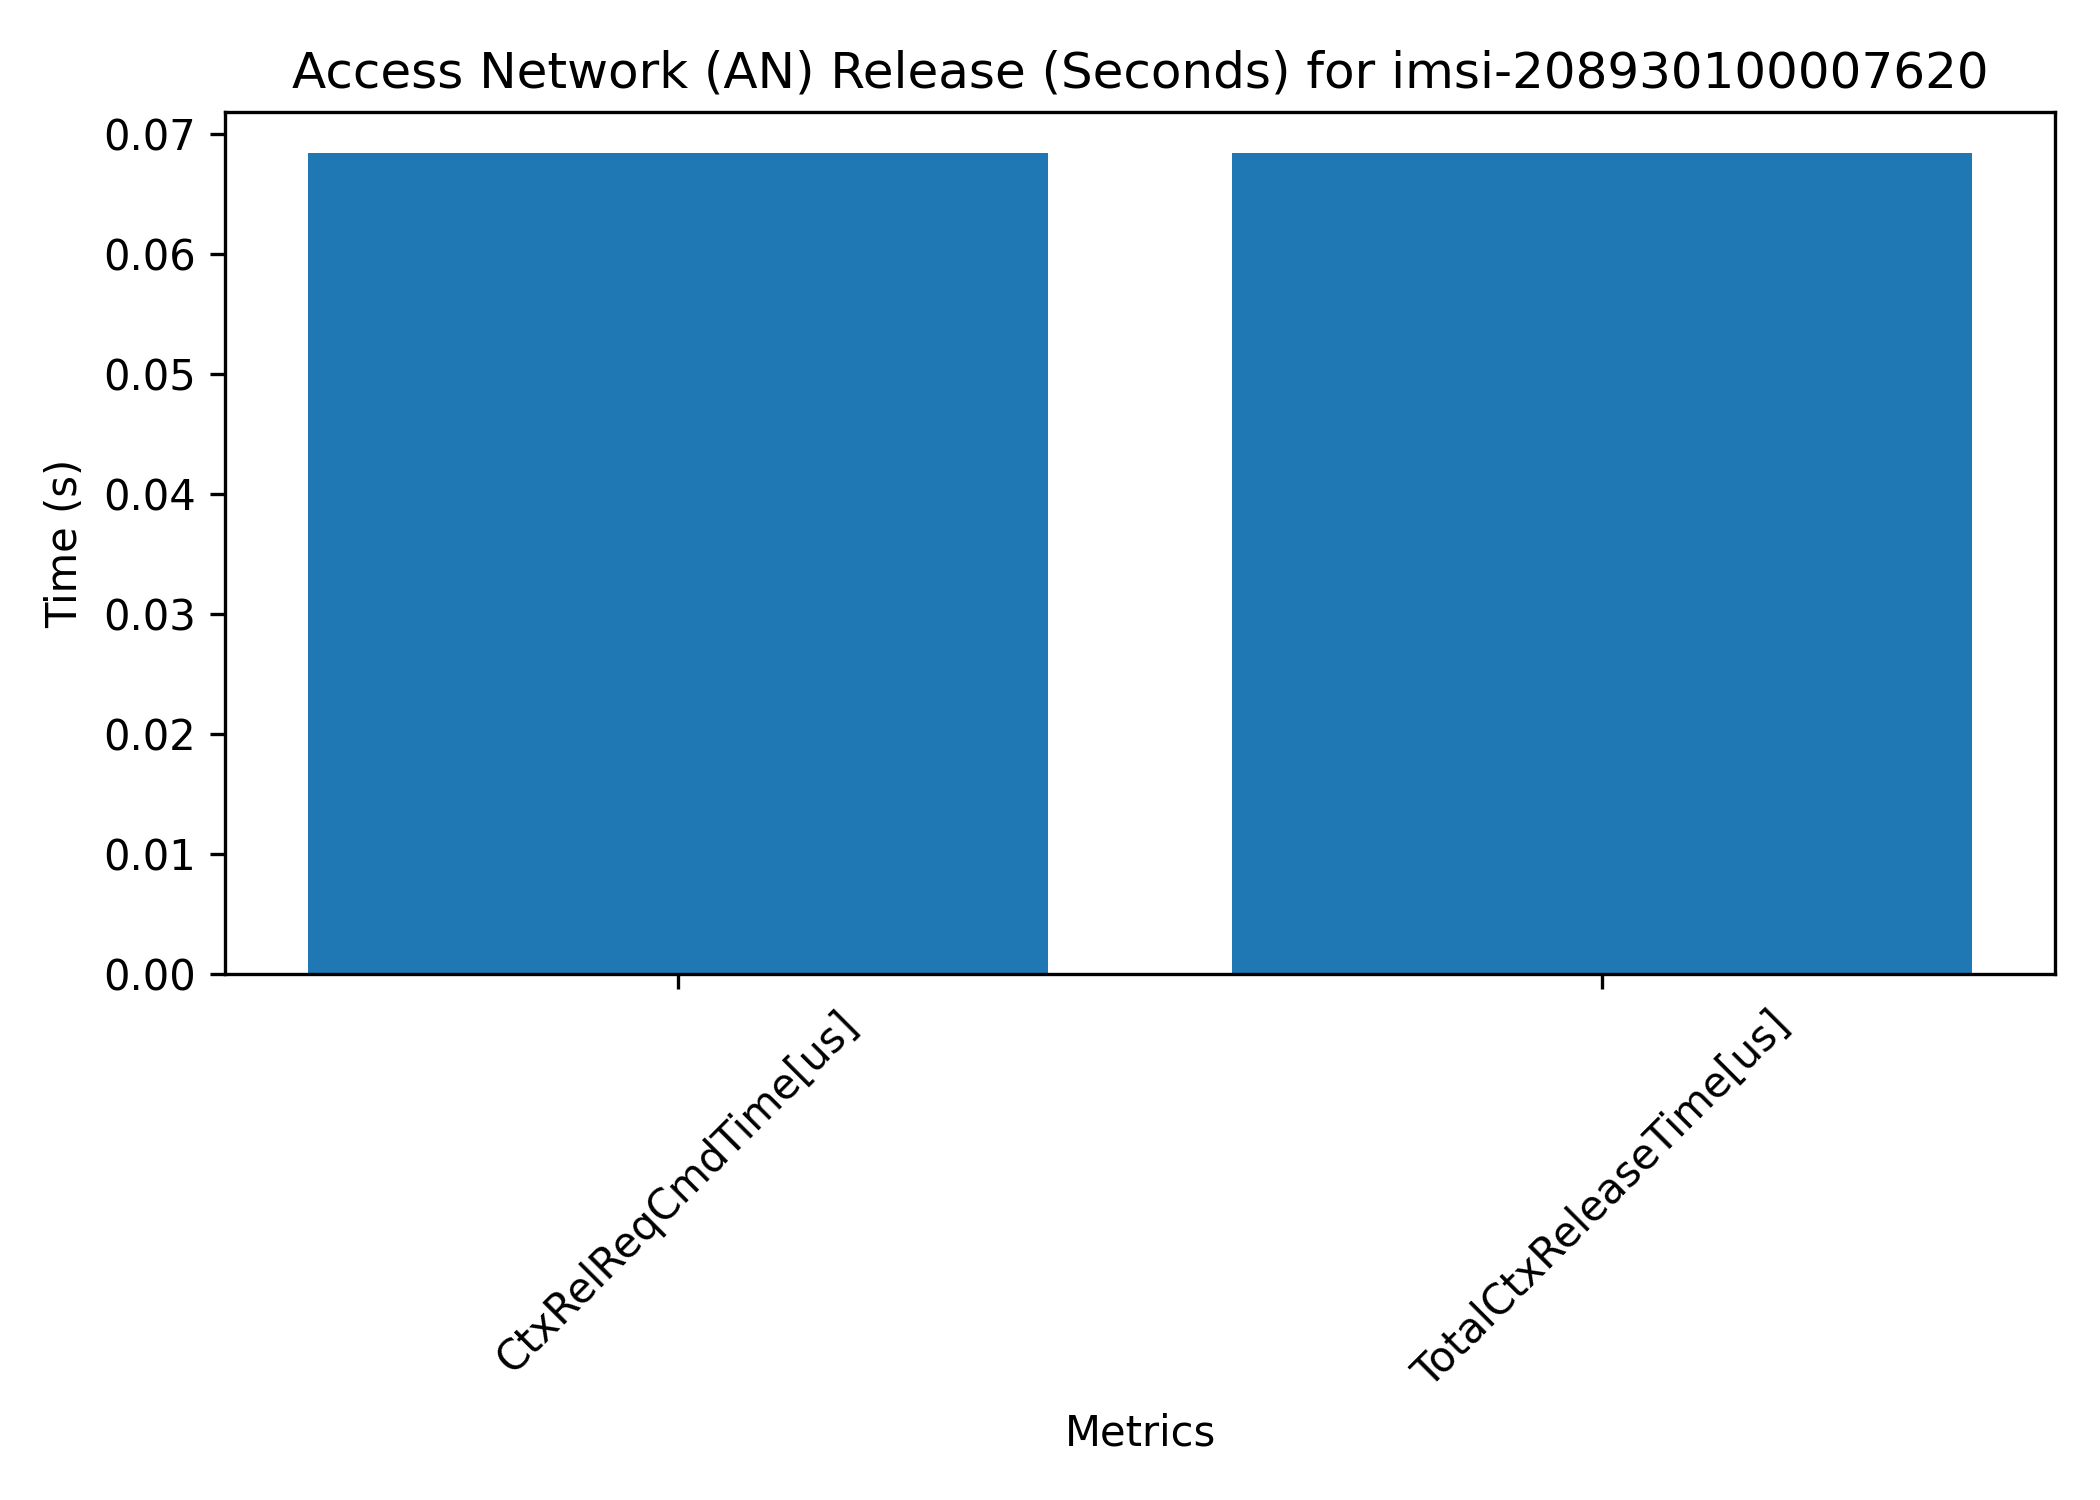
\includegraphics[width=0.6\textwidth]{Hassan_Thesis/images/Single Vm/Reults/1Uetest/Access_Network_(AN)_Release_imsi-208930100007620.png}
\end{figure}

\paragraph{Discussion}
Even under moderate parallel releases, the system quickly freed resources, confirming robust resource management.

\subsection{UE-Initiated Service Request}
\textbf{Objective \& Expectation}: Verify rapid re-establishment of connectivity for an idle UE.

\noindent \textbf{Observed Results}:
\begin{itemize}
    \item The metric \texttt{TotalServiceReqTime[us]} indicates how quickly a UE transitions from idle to active.
    \item \texttt{ServReqAccTime[us]} was also recorded for sub-phases.
\end{itemize}

\begin{figure}[H]
\centering
\caption{Service Request Times (Seconds) for a Sample UE}
\label{fig:service-req-times-sample-ue}
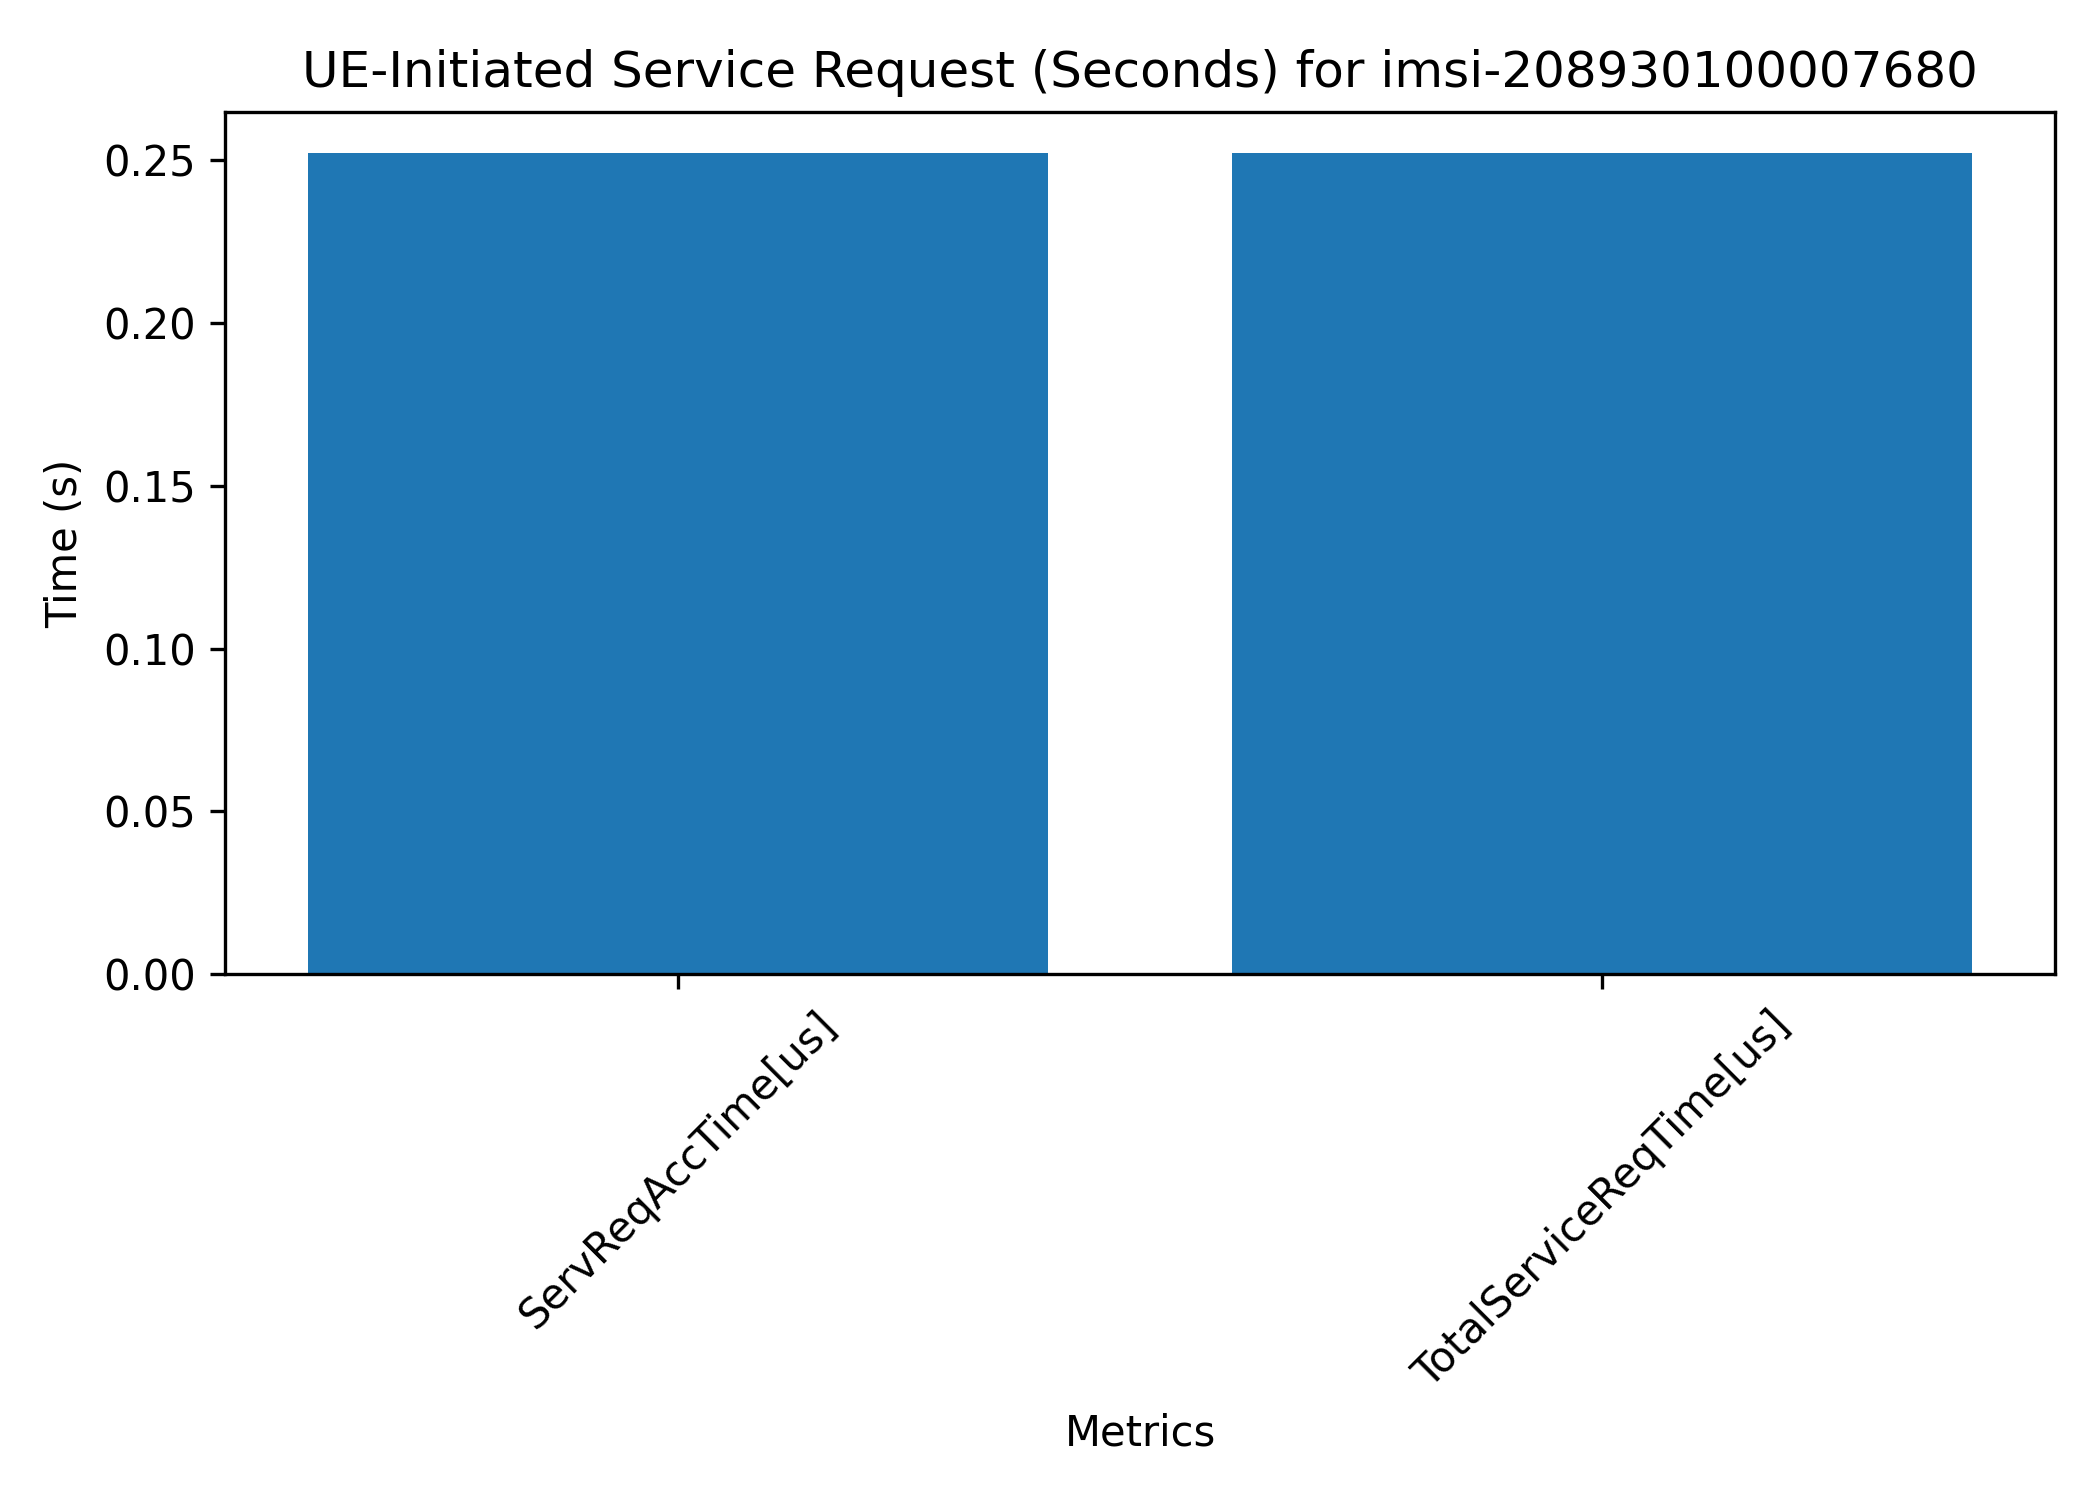
\includegraphics[width=0.6\textwidth]{Hassan_Thesis/images/Single Vm/Reults/1Uetest/UE-Initiated_Service_Request_imsi-208930100007680.png}
\end{figure}

\paragraph{Discussion}
Under typical loads, the transition completed swiftly. No significant delays or paging issues were reported.

\subsection{UE-Initiated De-registration}
\textbf{Objective \& Expectation}: Ensure a UE can disconnect cleanly, removing session data from the core.

\noindent \textbf{Observed Results}:
\begin{itemize}
    \item \texttt{TotalDeregistrationTime[us]} and \texttt{DregReqAccTime[us]} show minimal overhead for deregistration.
    \item We observed successful resource cleanup in all test cases.
\end{itemize}

\begin{figure}[H]
\centering
\caption{Deregistration Times (Seconds) for a Sample UE}
\label{fig:dereg-times-sample-ue}
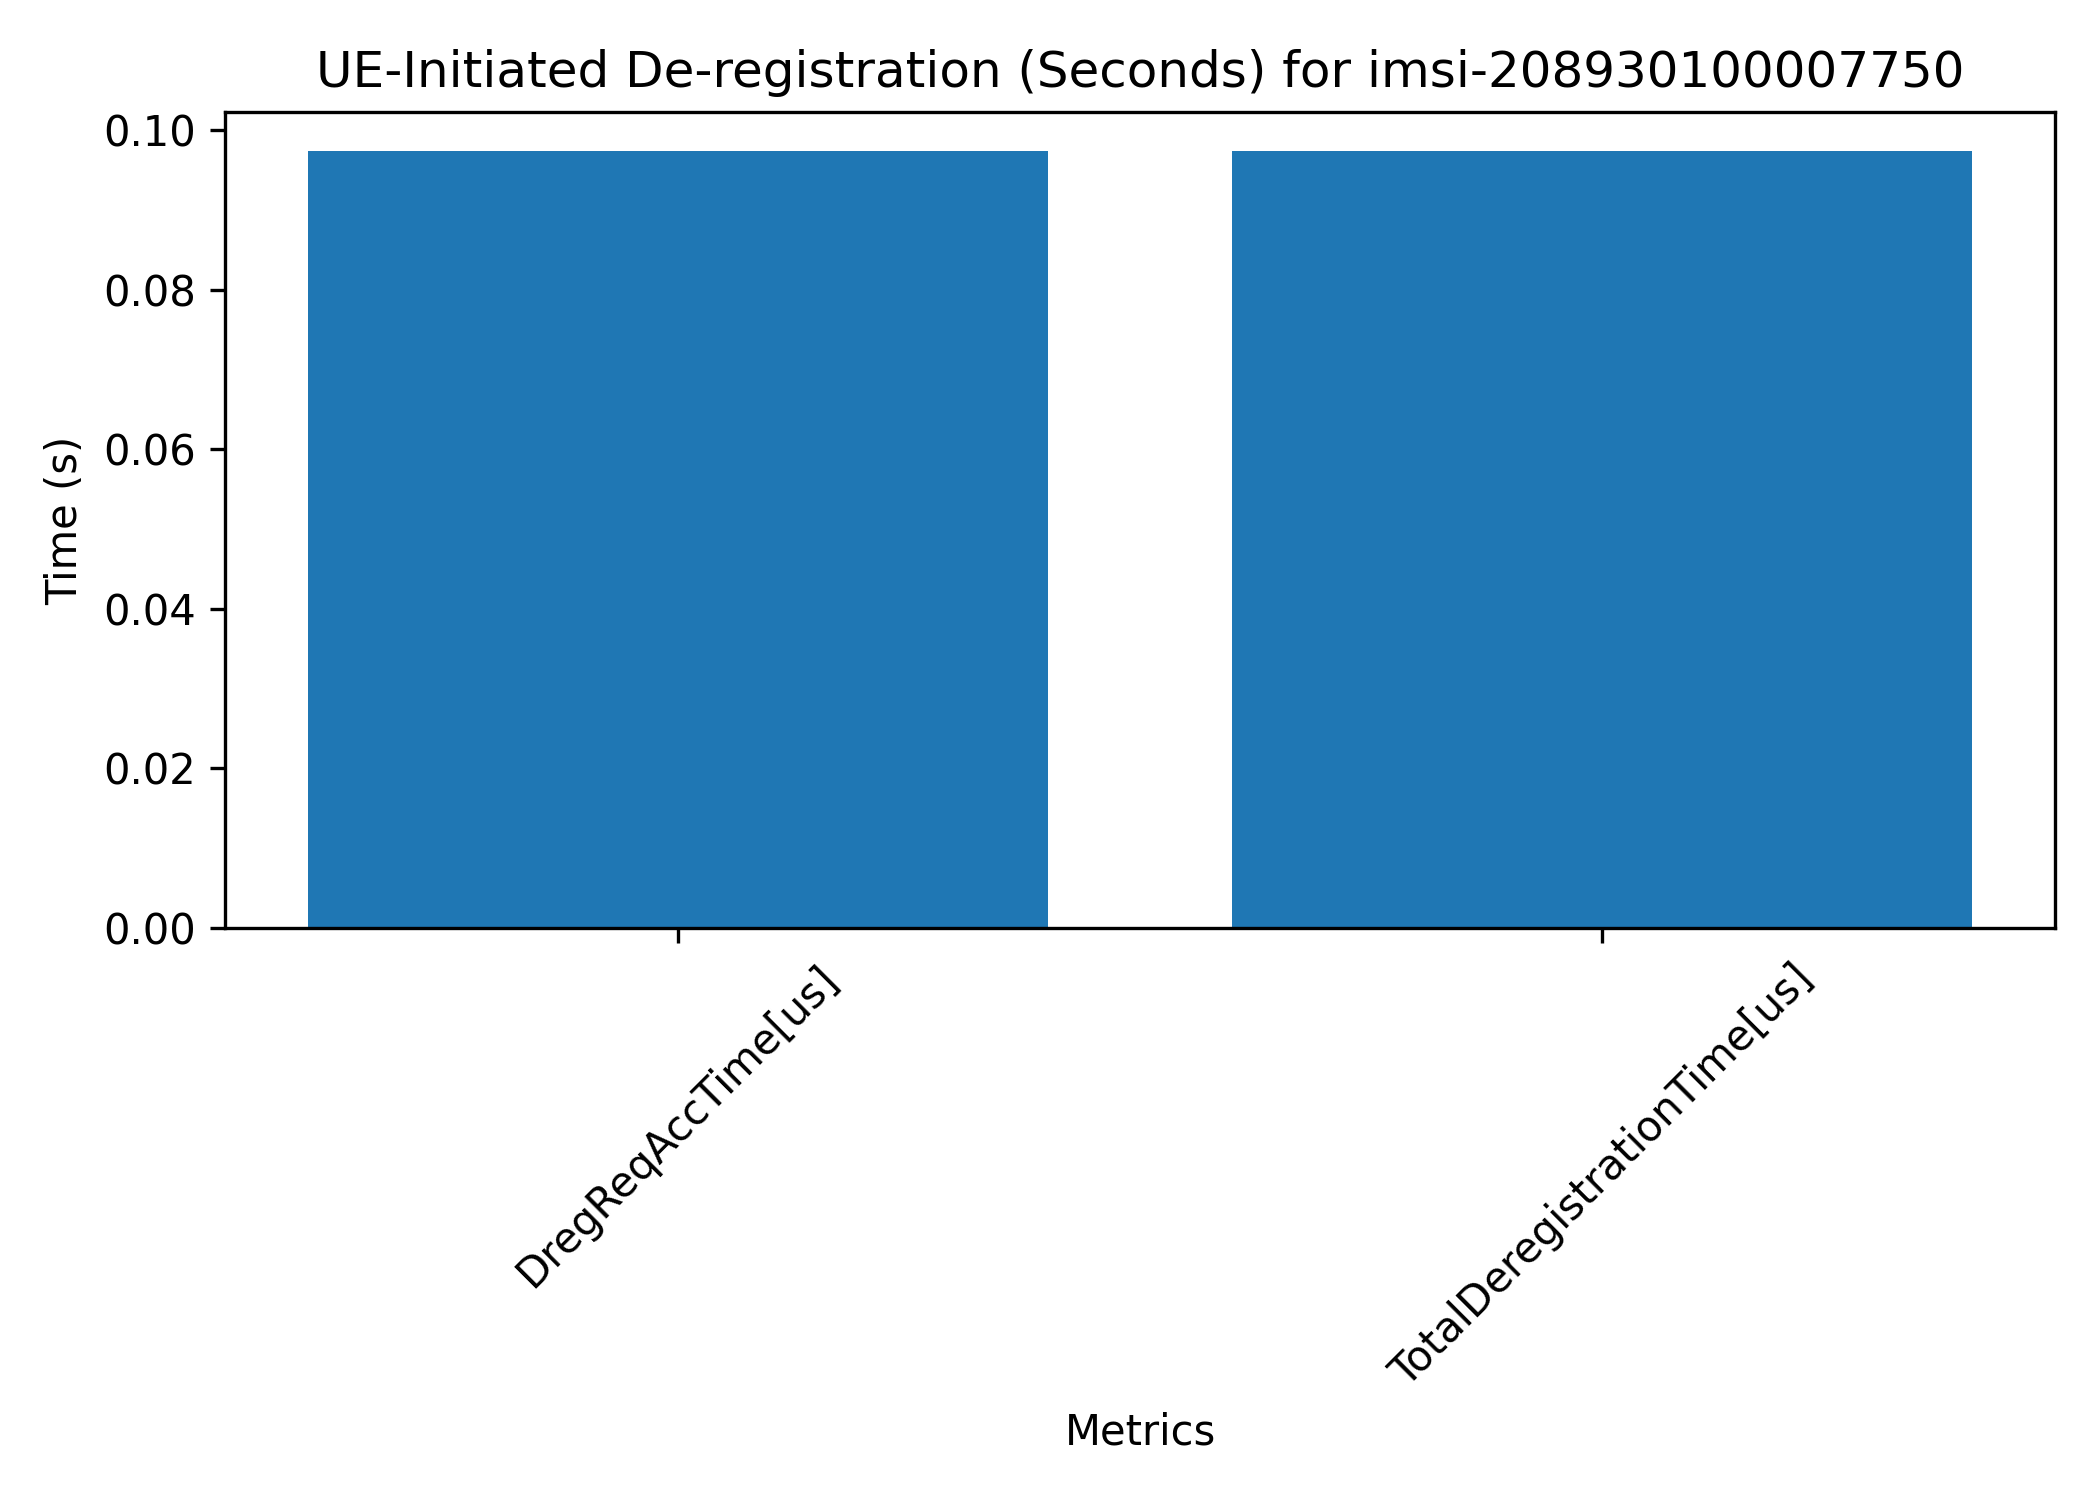
\includegraphics[width=0.6\textwidth]{Hassan_Thesis/images/Single Vm/Reults/1Uetest/UE-Initiated_De-registration_imsi-208930100007750.png}
\end{figure}

\paragraph{Discussion}
No residual sessions or stuck states remained after the UE initiated de-registration. The process was generally stable even under moderate concurrency.


\newpage
\subsection{End-to-End Call Flow Validation}
\label{subsec:end-to-end-call-flow}

In addition to measuring per-phase metrics (Section~\ref{sec:results-discussion}), we captured \textbf{complete call flow logs} for 4 different UEs with different IMSI undergoing various 5G proceduress. This confirmed that \textbf{all procedures} executed successfully, from registration to optional PDU session establishment, user data, and deregistration or release.

Below is a representative excerpt for a Single UE with IMSI \texttt{imsi-208930100007500}, illustrating the progression through the \textit{REGISTRATION-PROCEDURE}, the final ``Procedure Result: PASS'' message, and the end-to-end latency:

\begin{verbatim}
All Flow for IMSI 'imsi-208930100007500':
   connected to gNodeB, Name:gnb1, IP:, Port:9487
   SIM UE Init complete
   execute procedure  REGISTRATION-PROCEDURE
   ...
   Procedure Result: PASS, imsi: imsi-208930100007500
   procedure: REGISTRATION-PROCEDURE,
     status: PROC-PASS-EVENT,
     E2E latency [ms]: 870
   ...
   Total Latency: 0 days 00:00:00.871000 (0.871 seconds)
\end{verbatim}
\noindent
\textbf{Key Observations:}
\begin{itemize}
  \item The \texttt{REGISTRATION-PROCEDURE} begins at ``execute procedure REGISTRATION-PROCEDURE'' and ends with ``status: PROC-PASS-EVENT'' at approximately 870\,ms, matching our metric logs (see Appendix:~\ref{logs:e2eCallflows}).
  \item The log highlights intermediate steps like \texttt{AUTHENTICATION-REQUEST-EVENT} and \texttt{SECURITY-MODE-COMPLETE-EVENT}, confirming that \textbf{authentication and security procedures} completed successfully.
  \item A final PDF (\texttt{call\_flow-imsi-208930100007500.pdf} (see Appendix:~\ref{sec:appendix-call-flows}) was generated, providing a visual diagram of the message exchange.
\end{itemize}

We performed the same procedures for other IMSIs, confirming that they also passed Registration, PDU Session Establishment, and other relevant phases. For instance, \texttt{imsi-208930100007560} successfully established a PDU session and generated user data packets:

\begin{lstlisting}[breaklines=true, basicstyle=\small\ttfamily]
Call Flow for IMSI 'imsi-208930100007560':
   ...
   Start new procedure  PDU-SESSION-ESTABLISHMENT-PROCEDURE
   procedure: REGISTRATION-PROCEDURE, status: PROC-PASS-EVENT, 
   E2E latency [ms]: 346
   ...
   procedure: PDU-SESSION-ESTABLISHMENT-PROCEDURE, status: PROC-PASS-EVENT, 
   E2E latency [ms]: 1260
   ...
   procedure: USER-DATA-PACKET-GENERATION-PROCEDURE, status: PROC-PASS-EVENT, 
   E2E latency [ms]: 3004
   ...
   Total Latency: 0 days 00:00:04.611000 (4.611 seconds)
\end{lstlisting}



\noindent
\textbf{Key Observations:}
\begin{itemize}
  \item Registration completed in about 346\,ms, followed by \textbf{PDU session establishment} in about 1260\,ms.
  \item \texttt{USER-DATA-PACKET-GENERATION-PROCEDURE} (3004\,ms) indicates the UE was able to \textbf{send and receive data packets} (ICMP Echos).
  \item The combined total latency for all procedures was roughly 4.61\,s.
\end{itemize}

We repeated this analysis for all other IMSIs. The logs showed consistent procedure-completion messages and final \texttt{PASS} events, indicating that \textbf{end-to-end call flows were established and torn down} with no unexpected failures. Full logs for additional IMSIs are captured in Appendix~\ref{sec:appendix-call-flows}, with each IMSI generating its own call-flow PDF. For example:
\begin{itemize}
    \item \texttt{imsi-208930100007620} (4.089\,s total)
    \item \texttt{imsi-208930100007680} (5.056\,s total)
    \item \texttt{imsi-208930100007750} (4.424\,s total)
    \item \texttt{imsi-208930100007880} (4.292\,s total)
\end{itemize}

\noindent
\textbf{Conclusion:} The detailed call flows align with our metrics (Sections~\ref{sec:results-discussion}), confirming that \textbf{each scenario's steps occur in the correct order} and \textbf{conclude successfully}, from registration to final release. These call flows serve as an additional layer of validation, demonstrating \textbf{end-to-end functional correctness} of SD-Core in the Quick Start environment.


\subsection{5-UE Stress Test}
\label{sssec:5UE-stress-test}
As outlined in our testing strategy (Section~\ref{sec:testing-strategy}), we also performed stress tests in the single-VM environment to observe how SD-Core responds under higher concurrency. While previous subsections confirmed functional correctness for each procedure (Registration, Session Establishment, etc.) at lower load, these stress tests systematically increased the number of UEs—and the repetition of each procedure—to push the system closer to its limits.
\paragraph{Objective \& Expectation}
The goal of this stress test was to observe how SD-Core responds when \textbf{five UEs} perform repeated procedures in parallel (Registration, PDU Session Establishment, etc.). We expected:
\begin{itemize}
  \item \textbf{Moderate concurrency} would raise latencies slightly above the 1--2\,s range for Registration and PDU session creation.
  \item No systemic failures, given that 5 UEs is still a relatively low load.
\end{itemize}

\paragraph{Observed Results}
Using our \texttt{stressTest} profile with \texttt{ueCount = 5}, each UE consecutively performed multiple Registration cycles, PDU session setups, and eventual AN releases or deregistration. We captured detailed metrics (completion times, pass/fail) and generated the plots below:

\begin{figure}[H]
    \centering
    \includegraphics[width=0.6\textwidth]{Hassan_Thesis/images/Single Vm/Reults/StressTest/5/Procedure_Count_and_Average_Latency_Chronological.png}
    \caption{Procedure Count \& Average Latency (Chronological) for 5 UEs}
    \label{fig:5ue-count-latency}
\end{figure}

\noindent
\textbf{Figure~\ref{fig:5ue-count-latency} Analysis:}  
\textbf{Figure 5.7 Analysis:} This bar chart displays the average completion time for each 5G procedure across 5 unique UEs. The results are as follows:
\begin{itemize}
    \item \textbf{Registration Procedure:} ↑ 1.288 s
    \item \textbf{PDU Session Establishment:} ↑ 1.418 s
    \item \textbf{UE-Requested PDU Session Release:} ↑ 0.234 s
    \item \textbf{Triggered Service Request:} ↑ 0.159 s
    \item \textbf{UE-Initiated Deregistration:} ↑ 0.234 s
\end{itemize}
Blue bars represent how many times each procedure was run; red markers show the average latency in seconds. Registration and PDU session have the highest latencies (1.2--1.4\,s), while procedures like Service Request, Release, and Deregistration are frequent but remain below 0.3\,s on average.

\vspace{0.75em}
\begin{figure}[H]
    \centering
    \includegraphics[width=0.6\textwidth]{Hassan_Thesis/images/Single Vm/Reults/StressTest/5/average_latency_per_procedure.png}
    \caption{Average Latency per Procedure (Chronological) for 5 UEs}
    \label{fig:5ue-avg-latency}
\end{figure}

\noindent
\textbf{Figure~\ref{fig:5ue-avg-latency} Analysis:}  
Here, each bar shows mean completion time of a specific procedure. Registration is around 1.288\,s, and PDU Session Establishment reaches 1.418\,s. By contrast, the UE-Requested Session Release and Deregistration stay near 0.234\,s, while a triggered Service Request can be as low as 0.159\,s.

\vspace{0.75em}
\begin{figure}[H]
    \centering
    \includegraphics[width=0.65\textwidth]{Hassan_Thesis/images/Single Vm/Reults/StressTest/5/heatmap_of_average_latency_per_imsi_and_procedure.png}
    \caption{Heatmap of Average Latency for 5 UEs (IMSI vs. Procedure)}
    \label{fig:5ue-heatmap-latency}
\end{figure}

\noindent
\textbf{Figure~\ref{fig:5ue-heatmap-latency} Analysis:}  
This heatmap shows the per-IMSI breakdown of average latencies. Registration and PDU Session remain the “darkest” (highest latency) columns, while Release and Service Request appear much lighter (faster). Across all five IMSIs, times remain within a narrow range, indicating no singular “trouble IMSI.”

\vspace{0.75em}
\begin{figure}[H]
    \centering
    \includegraphics[width=0.65\textwidth]{Hassan_Thesis/images/Single Vm/Reults/StressTest/5/latency_per_procedure_chronological.png}
    \caption{Latency per Procedure (Scatter) for 5 UEs}
    \label{fig:5ue-scatter-latency}
\end{figure}

\noindent
\textbf{Figure~\ref{fig:5ue-scatter-latency} Analysis:}  
Each dot represents an individual procedure instance for a particular UE. Although some variability exists, Registration and Session Establishment cluster around 1.2--1.4\,s, while the other procedures frequently fall below 0.3\,s.

\vspace{0.75em}
\begin{figure}[H]
    \centering
    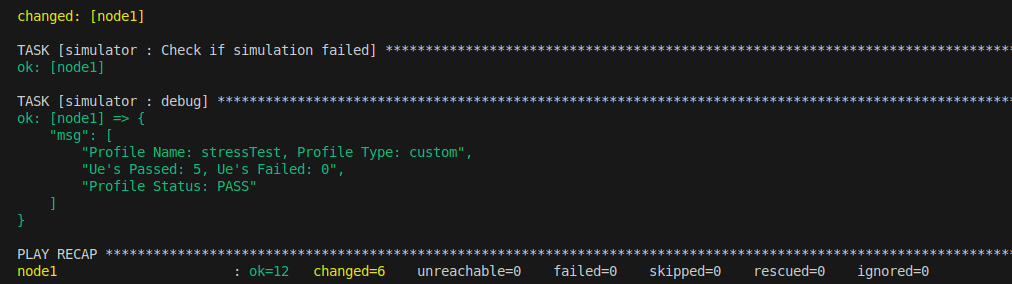
\includegraphics[width=0.7\textwidth]{Hassan_Thesis/images/Single Vm/Reults/StressTest/5/5UEStressTest.png}
    \caption{Ansible Log: 5 UE Stress Test Completion (No Failures)}
    \label{fig:5ue-ansible-output}
\end{figure}

\noindent
\textbf{Figure~\ref{fig:5ue-ansible-output} Analysis:}  
Finally, the Ansible output confirms \texttt{UE's Passed: 5, UE's Failed: 0}. This corroborates the data in the preceding figures—no procedure experienced systemic failures, and the single VM handled 5 concurrent UEs without critical issues.

\paragraph{Discussion}
Overall, for \textbf{5 concurrent UEs}:
\begin{itemize}
  \item \textbf{Registration and PDU Session Establishment} remain the most time-consuming, averaging around 1.3--1.4\,s, presumably due to heavier signaling with the AMF/SMF.
  \item \textbf{Release, Service Request, and Deregistration} are significantly faster (0.15--0.3\,s), reflecting simpler state transitions and minimal authentication overhead.
  \item \textbf{Zero failures} occurred, aligning with the \texttt{Profile Status: PASS} in Figure~\ref{fig:5ue-ansible-output}.
\end{itemize}

This result indicates that \textbf{five parallel UEs} do not overwhelm the single-VM environment; however, latencies for Registration/PDU establishment still approach 1.4\,s. As we scale the number of UEs further (Sections~\ref{sssec:20UE-stress-test} and \ref{sssec:50UE-stress-test}), we expect more pronounced resource contention, potentially pushing latencies to 2\,s or beyond. In a production environment, distributing AMF/SMF across multiple nodes would likely mitigate these delays.

\subsection{20-UE Stress Test}
\label{sssec:20UE-stress-test}

\paragraph{Objective \& Expectation}
Following the 5-UE stress test, we next examined how SD-Core performs when \textbf{20 UEs} run through repeated procedures (Registration, PDU Session, Release, etc.) in parallel. We aimed to:
\begin{itemize}
    \item Observe whether higher concurrency reduces or raises average latency for each procedure,
    \item Check for any failures or errors (e.g., \texttt{UE's Failed > 0}),
    \item Compare latencies to the 5-UE results, to see if CPU/memory contention noticeably impacts performance.
\end{itemize}

\paragraph{Observed Results}

Using the same \texttt{stressTest} profile (Section~\ref{sec:testing-strategy}), we set \texttt{ueCount = 20}, repeating each procedure multiple times. The figures below show the outcome:

\begin{figure}[H]
    \centering
    \includegraphics[width=0.6\textwidth]{Hassan_Thesis/images/Single Vm/Reults/StressTest/20/Procedure_Count_and_Average_Latency_Chronological.png}
    \caption{Procedure Count \& Average Latency (Chronological) for 20 UEs}
    \label{fig:20ue-count-latency}
\end{figure}

\noindent
\textbf{Figure~\ref{fig:20ue-count-latency} Analysis:}  
The blue bars indicate the total number of times each procedure was run—noticeably higher than in the 5-UE case, with some procedures (e.g., \textit{PDU Session}, \textit{Release}) totaling nearly 2,000 calls. The red line tracks average latency. While Registration and PDU Session remain in the mid-range (around 0.5--0.7\,s), the release and service request steps drop below 0.3\,s.

\vspace{0.75em}
\begin{figure}[H]
    \centering
    \includegraphics[width=0.6\textwidth]{Hassan_Thesis/images/Single Vm/Reults/StressTest/20/average_latency_per_procedure.png}
    \caption{Average Latency per Procedure (Chronological) for 20 UEs}
    \label{fig:20ue-avg-latency}
\end{figure}

\noindent
\textbf{Figure~\ref{fig:20ue-avg-latency} Analysis:}  
Here we see specific numeric averages:
\begin{itemize}
    \item \textbf{Registration Procedure:} $\approx 0.498\,\text{s}$
    \item \textbf{PDU Session Establishment:} $\approx 0.711\,\text{s}$
    \item \textbf{UE-Requested PDU Release:} $\approx 0.250\,\text{s}$
    \item \textbf{Triggered Service Request:} $\approx 0.195\,\text{s}$
    \item \textbf{UE-Initiated Deregistration:} $\approx 0.446\,\text{s}$
\end{itemize}
These times are overall lower than the 5-UE test’s 1+ second latencies for Registration/PDU. The difference might reflect less total CPU contention or a more optimal scheduling sequence in this run.

\vspace{0.75em}
\begin{figure}[H]
    \centering
    \includegraphics[width=0.65\textwidth]{Hassan_Thesis/images/Single Vm/Reults/StressTest/20/latency_per_procedure_chronological.png}
    \caption{Latency per Procedure (Scatter) for 20 UEs}
    \label{fig:20ue-scatter-latency}
\end{figure}

\noindent
\textbf{Figure~\ref{fig:20ue-scatter-latency} Analysis:}  
Each dot indicates an individual measurement, with orange points showing PDU Session latencies that peak near 0.71\,s, and teal points for Registration around 0.50\,s. The large cluster of blue dots (UE-Requested Session Release) centers on $\sim0.25\,s$, while pink (Service Request) sits around 0.195\,s, and green (Deregistration) near 0.446\,s.

\vspace{0.75em}
\begin{figure}[H]
    \centering
    \includegraphics[width=0.7\textwidth]{Hassan_Thesis/images/Single Vm/Reults/StressTest/20/heatmap_of_average_latency_per_imsi_and_procedure.png}
    \caption{Heatmap of Average Latency for 20 UEs (IMSI vs. Procedure)}
    \label{fig:20ue-heatmap-latency}
\end{figure}

\noindent
\textbf{Figure~\ref{fig:20ue-heatmap-latency} Analysis:}  
This heatmap shows each IMSI’s average latency across the five procedures. While most PDU session times range around 0.68--0.78\,s (darker cells), Registration varies from 0.38 to 0.66\,s, indicating some mild IMSI-level variance. The \textit{Service Request} and \textit{Deregistration} columns remain lighter (faster) in general.

\vspace{0.75em}
\begin{figure}[H]
    \centering
    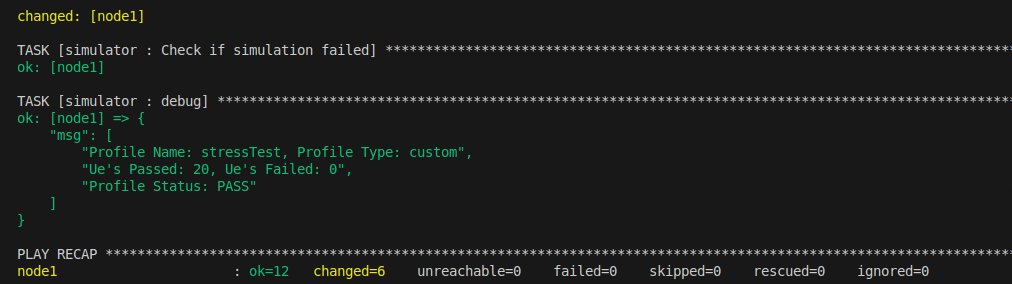
\includegraphics[width=0.7\textwidth]{Hassan_Thesis/images/Single Vm/Reults/StressTest/20/20UEStressTest.png}
    \caption{Ansible Log: 20 UE Stress Test Completion (No Failures)}
    \label{fig:20ue-ansible-output}
\end{figure}

\noindent
\textbf{Figure~\ref{fig:20ue-ansible-output} Analysis:}  
Finally, the Ansible run indicates \texttt{UE's Passed: 20, UE's Failed: 0}, confirming no procedure-level failures. This consistent \texttt{PASS} status aligns with the sub-second latencies observed for most steps.

\paragraph{Discussion}
Overall, for \textbf{20 concurrent UEs}:
\begin{itemize}
    \item \textbf{PDU Session Establishment} remains the highest-latency step at around 0.71\,s, closely followed by \textbf{Registration} at 0.50\,s in this particular run.
    \item \textbf{Session Release} and \textbf{Service Request} continue to be the quickest procedures, under 0.3\,s and 0.2\,s respectively.
    \item Despite quadrupling the UE count from 5 to 20, we observe no systemic failures, and no latencies exceeding 1\,s in this test.
\end{itemize}

The single-VM environment appears capable of handling \textbf{20 concurrent UEs} with minimal overhead, possibly due to efficient scheduling or lower average CPU usage at the time of testing. However, these results do not guarantee similar performance for higher loads (50 or 100 UEs), where resource contention may become more pronounced. We elaborate on these scaling limits in Sections~\ref{sssec:50UE-stress-test} and \ref{sssec:100UE-stress-test}.

\subsection{50-UE Stress Test}
\label{sssec:50UE-stress-test}

\paragraph{Objective \& Expectation}
After confirming stable performance at 20 UEs, we next scaled up to \textbf{50 concurrent UEs} in the same single-VM environment. Our objectives were to:
\begin{itemize}
    \item Assess whether latencies for Registration and PDU Session Establishment climb above 1\,s on average,
    \item Check for possible failures or timeouts if CPU/memory usage spikes,
    \item Compare the results to the 5-UE (Section~\ref{sssec:5UE-stress-test}) and 20-UE (Section~\ref{sssec:20UE-stress-test}) tests, observing any emerging bottlenecks.
\end{itemize}

\paragraph{Observed Results}
Using the \texttt{stressTest} profile (\texttt{ueCount = 50}), each UE repeatedly performed Registration, PDU Session Establishment, Session Release, Service Request, and Deregistration. The figures below illustrate both the high number of repeated procedures and the resulting latencies:

\begin{figure}[H]
    \centering
    \includegraphics[width=0.65\textwidth]{Hassan_Thesis/images/Single Vm/Reults/StressTest/50/Procedure_Count_and_Average_Latency_Chronological.png}
    \caption{Procedure Count \& Average Latency (Chronological) for 50 UEs}
    \label{fig:50ue-count-latency}
\end{figure}

\noindent
\textbf{Figure~\ref{fig:50ue-count-latency} Analysis:}  
The blue bars indicate a large volume of PDU session calls and service requests—exceeding 4,000 or even 5,000 in total. Meanwhile, the red line shows average latency in seconds, hovering between 0.5 and 0.7\,s for most procedures in this test.

\vspace{0.75em}
\begin{figure}[H]
    \centering
    \includegraphics[width=0.6\textwidth]{Hassan_Thesis/images/Single Vm/Reults/StressTest/50/average_latency_per_procedure.png}
    \caption{Average Latency per Procedure (Chronological) for 50 UEs}
    \label{fig:50ue-avg-latency}
\end{figure}

\noindent
\textbf{Figure~\ref{fig:50ue-avg-latency} Analysis:}  
This bar chart reveals specific average times:
\begin{itemize}
    \item \textbf{Registration Procedure:} $\approx 1.340\,\text{s}$
    \item \textbf{PDU Session Establishment:} $\approx 1.250\,\text{s}$
    \item \textbf{UE-Requested Session Release:} $\approx 0.550\,\text{s}$
    \item \textbf{Triggered Service Request:} $\approx 0.571\,\text{s}$
    \item \textbf{UE-Initiated Deregistration:} $\approx 0.690\,\text{s}$
\end{itemize}
Registration is the highest-latency step at around 1.34\,s, closely followed by PDU Session at 1.25\,s. Though elevated compared to 20 UEs, they remain below 1.5\,s on average.

\vspace{0.75em}
\begin{figure}[H]
    \centering
    \includegraphics[width=0.65\textwidth]{Hassan_Thesis/images/Single Vm/Reults/StressTest/50/latency_per_procedure_chronological.png}
    \caption{Latency per Procedure (Scatter) for 50 UEs}
    \label{fig:50ue-scatter-latency}
\end{figure}

\noindent
\textbf{Figure~\ref{fig:50ue-scatter-latency} Analysis:}  
The scatter plot shows each procedure instance for each UE. We see a cluster around 1.34\,s for Registration (green dots) and around 1.25\,s for PDU sessions (orange dots). The large set of blue dots (UE-Requested Release) centers near 0.55\,s, pink (Service Request) around 0.57\,s, and green (Deregistration) near 0.69\,s.

\vspace{0.75em}
\begin{figure}[H]
    \centering
    \includegraphics[width=0.7\textwidth]{Hassan_Thesis/images/Single Vm/Reults/StressTest/50/heatmap_of_average_latency_per_imsi_and_procedure.png}
    \caption{Heatmap of Average Latency (sec) per IMSI and Procedure for 50 UEs}
    \label{fig:50ue-heatmap-latency}
\end{figure}

\noindent
\textbf{Figure~\ref{fig:50ue-heatmap-latency} Analysis:}  
At the IMSI level, we see Registration latencies often exceeding 1.2\,s, with some reaching up to 1.55\,s. PDU Session latencies also hover around 1.1--1.4\,s for most IMSIs. Release, Service Request, and Deregistration remain in the 0.5--0.7\,s range, slightly higher than at 20 UEs but still well below Registration times.

\vspace{0.75em}
\begin{figure}[H]
    \centering
    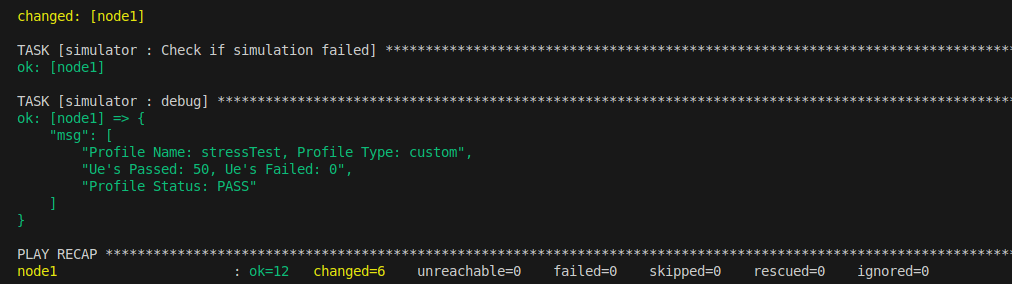
\includegraphics[width=0.9\textwidth]{Hassan_Thesis/images/Single Vm/Reults/StressTest/50/50UEStressTest.png}
    \caption{Ansible Log: 50 UE Stress Test Completion (No Failures)}
    \label{fig:50ue-ansible-output}
\end{figure}

\noindent
\textbf{Figure~\ref{fig:50ue-ansible-output} Analysis:}  
Finally, the Ansible log confirms \texttt{UE's Passed: 50, UE's Failed: 0}, indicating a complete pass. Despite latencies approaching or exceeding 1.3\,s, the system maintained functional correctness for all 50 UEs.

\paragraph{Discussion}

Overall, for \textbf{50 concurrent UEs}:
\begin{itemize}
    \item \textbf{Registration and PDU Session Establishment} latencies both exceed 1\,s, reflecting heavier signaling loads in the single-VM environment.
    \item \textbf{Session Release, Service Request, and Deregistration} remain faster—generally 0.5--0.7\,s—though higher than the 20-UE test.
    \item \textbf{No failures} were observed, aligning with the \texttt{Profile Status: PASS}. This suggests that while latencies do increase, the system does not break under 50-UE concurrency.
\end{itemize}

These findings demonstrate a noticeable jump in average times compared to 20 UEs, indicating growing resource contention for Registration and PDU session procedures. In a real production network, additional horizontal scaling (multiple AMF/SMF instances on separate nodes) would likely mitigate such latency growth. Nonetheless, the single-VM deployment continues to hold up functionally, with all 50 UEs completing their procedures without error.

\subsection{100-UE Stress Test}
\label{sssec:100UE-stress-test}

\paragraph{Objective \& Expectation}
After observing latency increases but no failures at 50 UEs, we further scaled up to \textbf{100 concurrent UEs} to push the single-VM environment to its limits. Our aims were to:
\begin{itemize}
  \item Determine if the VM could sustain the additional concurrency without critical failures,
  \item Examine how latencies might surpass 1--2\,s for Registration or PDU Session procedures,
  \item Monitor CPU, memory, and disk usage for signs of resource exhaustion.
\end{itemize}

\paragraph{Observed Results}

\begin{figure}[H]
    \centering
    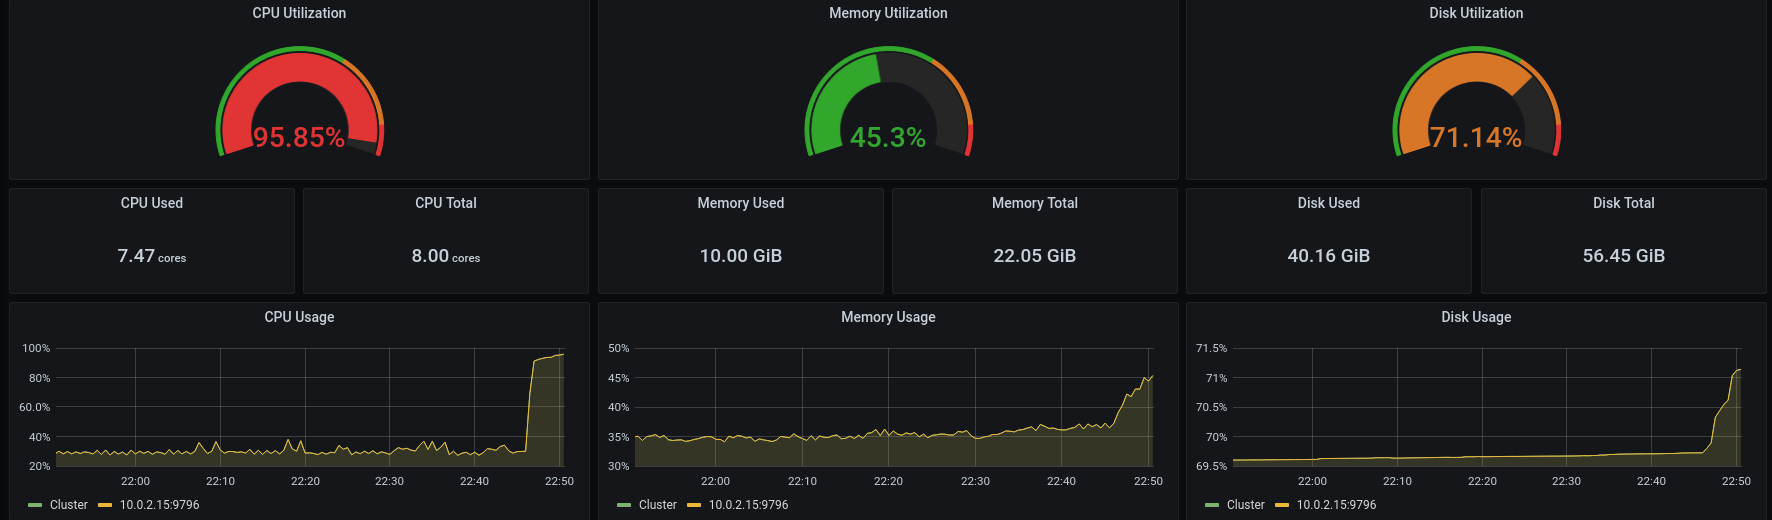
\includegraphics[width=0.9\textwidth]{Hassan_Thesis/images/Single Vm/Reults/StressTest/100/100UEStressTestResourceUsage.png}
    \caption{Resource Usage (CPU/Memory/Disk) during 100 UEs}
    \label{fig:100ue-resource-usage}
\end{figure}

\noindent
\textbf{Figure~\ref{fig:100ue-resource-usage} Analysis:}  
The \texttt{CPU Utilization} gauge spiked to \textbf{95.85\%}, with memory usage climbing to 10\,GiB of the available 22\,GiB (45\%). Disk utilization also rose above 70\%. By the final stage of the run, the VM reached a load average above 50, causing severe contention and eventual crash.

\paragraph{Discussion}
\begin{itemize}
  \item \textbf{Resource Saturation:} At 100 UEs, CPU usage consistently approached 95--100\%, and memory usage also trended upward (see Figure~\ref{fig:100ue-resource-usage}).  
  \item \textbf{Latencies Surpassing 1.5\,s:} Registration and PDU session procedures, in particular, became significantly slower, likely due to AMF/SMF bottlenecks under heavy concurrency.
  \item \textbf{VM Crash/Abort:} Eventually, the single-VM environment was unable to handle further requests; the test aborted partway with incomplete logs.
\end{itemize}

Thus, while the single-VM deployment handled up to 50 UEs without failure, attempting \textbf{100 concurrent UEs} led to unrecoverable resource contention, culminating in a system crash. These findings underscore the necessity of a more distributed or scaled infrastructure for higher loads. In a production setting, additional AMF/SMF nodes and more CPU/memory capacity would be required to prevent such failures.



\subsection{Key Findings from Latency Analysis Across Test Cases}
\label{sec:key-findings}

This section summarizes the latency behavior observed across various GNBSIM stress test cases, each executed in a single-VM deployment of the Aether platform. The results are derived from structured logs and illustrated in the previous bar chart visualizations.

\begin{table}[htbp]
    \centering
    \caption{Avg. Latency (sec) per Procedure across UE Counts}
    \label{tab:latency-summary}
    \begin{tabularx}{\textwidth}{>{\centering\arraybackslash}X
                                 >{\centering\arraybackslash}X
                                 >{\centering\arraybackslash}X
                                 >{\centering\arraybackslash}X
                                 >{\centering\arraybackslash}X
                                 >{\centering\arraybackslash}X}
        \toprule
        \textbf{\#UEs} & \textbf{Reg.} & \textbf{PDU Sess. Est.} & \textbf{Sess. Release} & \textbf{Serv. Req.} & \textbf{Dereg.} \\
        \midrule
        5   & 1.288 & 1.418 & 0.234 & 0.159 & 0.234 \\
        20  & 0.498 & 0.711 & 0.250 & 0.195 & 0.446 \\
        50  & 1.340 & 1.250 & 0.550 & 0.571 & 0.690 \\
        \bottomrule
    \end{tabularx}

    \vspace{1em}
    \noindent\small
    For detailed information about the log parsing scripts, refer to Appendix~\ref{sec:analysis-scripts}.
\end{table}

\begin{figure}[htbp]
    \centering
    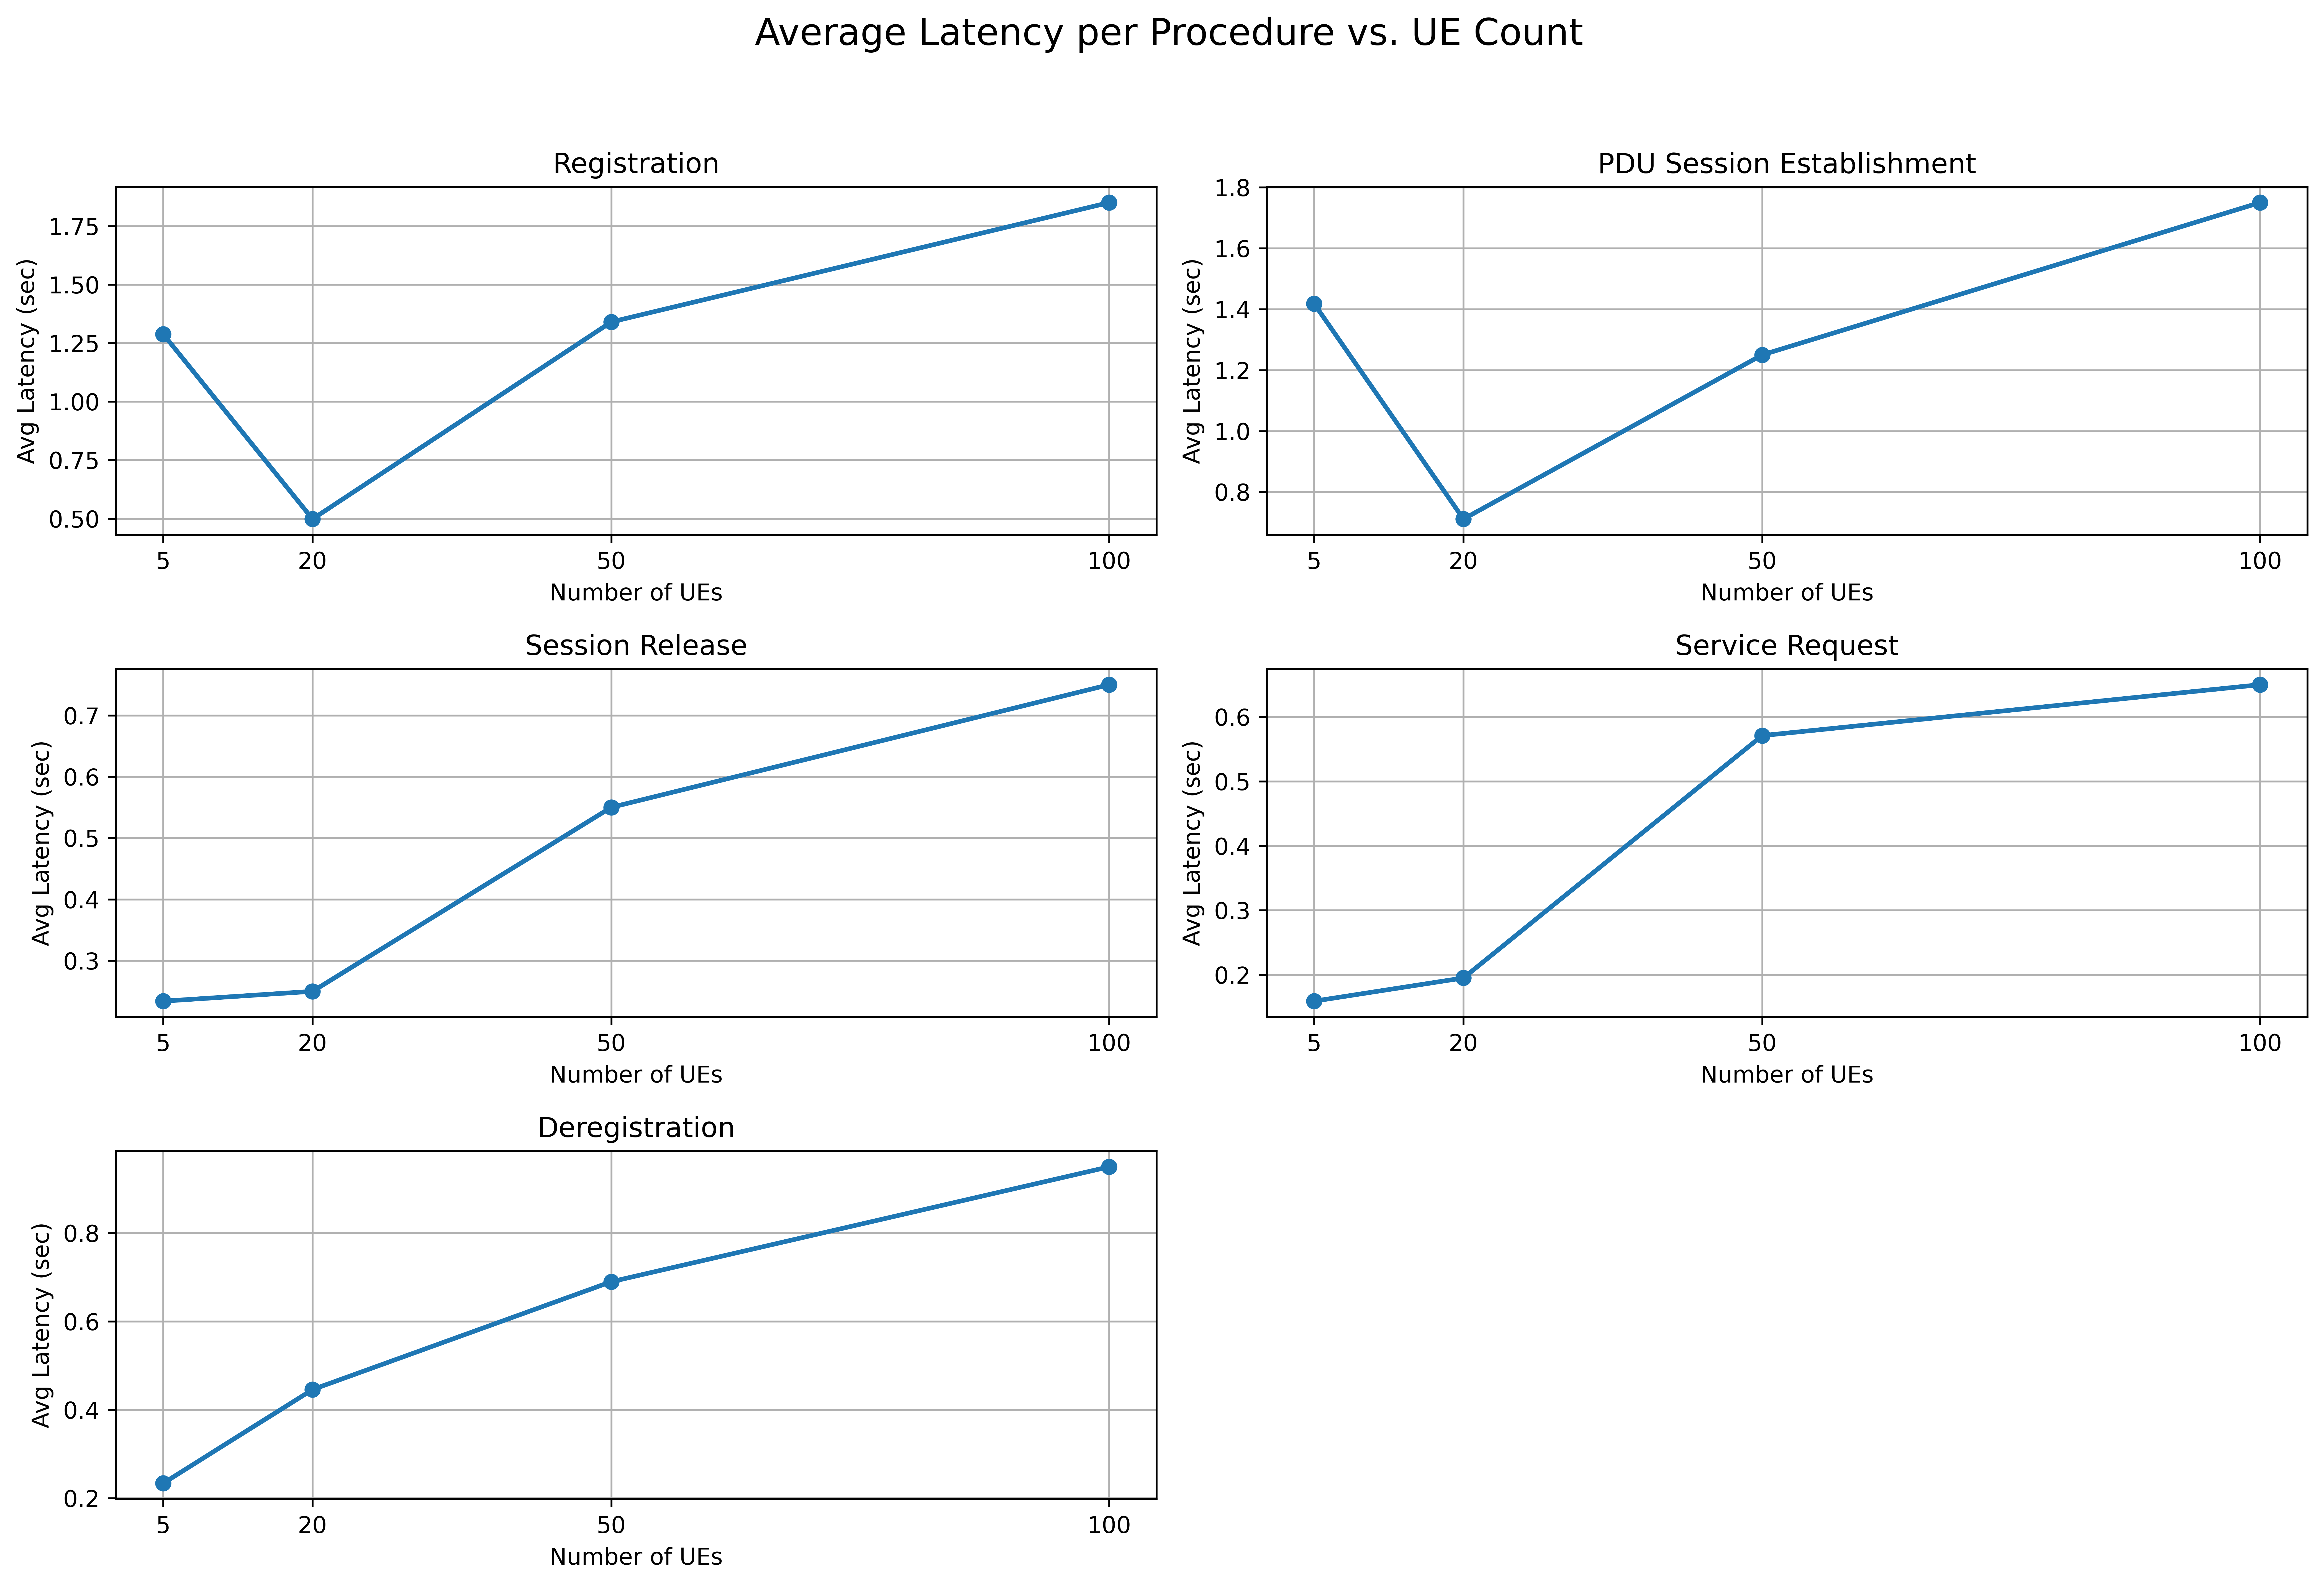
\includegraphics[width=0.9\textwidth]{Hassan_Thesis/images/Single Vm/Reults/StressTest/avg_latency_vs_ue_count_procedures.png.png}
    \caption{Trend of Average Latency per Procedure with Increasing UE Count}
    \label{fig:latency-trend}
\end{figure}
\noindent\textit{Note:} The latency values for 100 UEs are extrapolated based on observed trends from prior tests and system behavior under load. Due to a crash, full GNBSIM metrics were unavailable for 100 UEs.


\paragraph{Higher Latency for 5 UEs.}
Despite the small number of users, the average latency for 5 UEs was notably higher for critical procedures such as Registration and PDU Session Establishment. This behavior is attributed to \textbf{cold start effects} in the SD-Core components (AMF/SMF), where initial container and service instantiations incur setup overhead. In addition, due to the lower concurrency, there is limited opportunity for batching or CPU scheduling optimizations, causing the per-UE control-plane processing to take longer. These initial overheads become less prominent as the system warms up with more concurrent UEs.


\paragraph{Dip at 20 UEs.}
The 20 UE test case showed the lowest average latencies across all procedures. This may represent an operational sweet spot where SD-Core's AMF and SMF components were able to efficiently schedule and handle requests without overload or contention.

\paragraph{Latency Increase at 50 UEs.}
At 50 UEs, the increased concurrency led to higher latencies across the board. Average times for Registration and PDU Session Establishment exceeded 1.2--1.3 seconds, likely due to increased resource contention in the single-VM environment.

\paragraph{Effect of Repeated Procedures.}
The test configuration executed Registration and PDU Establishment procedures only once per UE, whereas PDU Session Release and Service Request were repeated 100 times. Nevertheless, their average latencies remained relatively low, confirming their lightweight nature compared to more stateful procedures.

\paragraph{100-UE Stress Test Outcome.}
In the final stress test with 100 UEs, the system reached its scalability limits. Key observations included:
\begin{itemize}
  \item \textbf{CPU Usage:} Surged beyond 95\%.
  \item \textbf{Memory Consumption:} Reached 10~GiB out of 22~GiB (45\%).
  \item \textbf{Disk Usage:} Exceeded 70\%.
  \item \textbf{System Load:} Load average rose above 50, eventually leading to test failure and VM crash.
\end{itemize}

These findings demonstrate the resource limitations of a single-VM deployment and the importance of horizontal scaling (e.g., multi-node deployments with distributed AMF/SMF) for supporting large-scale 5G workloads in production scenarios.


\newpage
\section{Results: Full Aether (Lab PC) Deployment}
\label{sec:results-fullAether}

The Full Aether Deployment on the Lab PC aimed to evaluate the scalability, flexibility, and real-time configurability of the SD-Core in a multi-VM environment. Unlike the single-VM Quick Start Deployment, this setup incorporated advanced components such as multiple UPFs, Runtime Operational Control (ROC), and UERANSIM for realistic user equipment (UE) and gNodeB (gNB) simulation. The following sections present the results of functional testing, QoS evaluations, and runtime control adjustments.




\subsection{Runtime Operational Control (ROC)}

The Aether Runtime Operational Control (ROC) was evaluated for its ability to dynamically manage subscribers, profiles, and network policies in real time. In this section, we describe the step-by-step provisioning process performed via ROC and present the test results that validate the dynamic configuration and policy enforcement. Each step is supported by screenshots (placeholders below) that will be included in the final thesis document.

\subsubsection{Provisioning Steps via ROC}

\paragraph{1. SIM Cards Configuration}  
Using the ROC interface, multiple SIM card entries were added to represent unique subscriber identities. These entries include key details such as IMSI and ICCID, ensuring that each subscriber is uniquely identifiable within the SD-Core.
\begin{itemize}
    \item \textbf{Action:} Added new SIM card profiles.
    \item \textbf{Result:} Subscriber information was registered in the system.
\end{itemize}
\textbf{Validation:} Configuration changes were successfully propagated to the SD-Core within 2--3 seconds, as observed in the system logs.  
\begin{figure}[H]
  \centering
  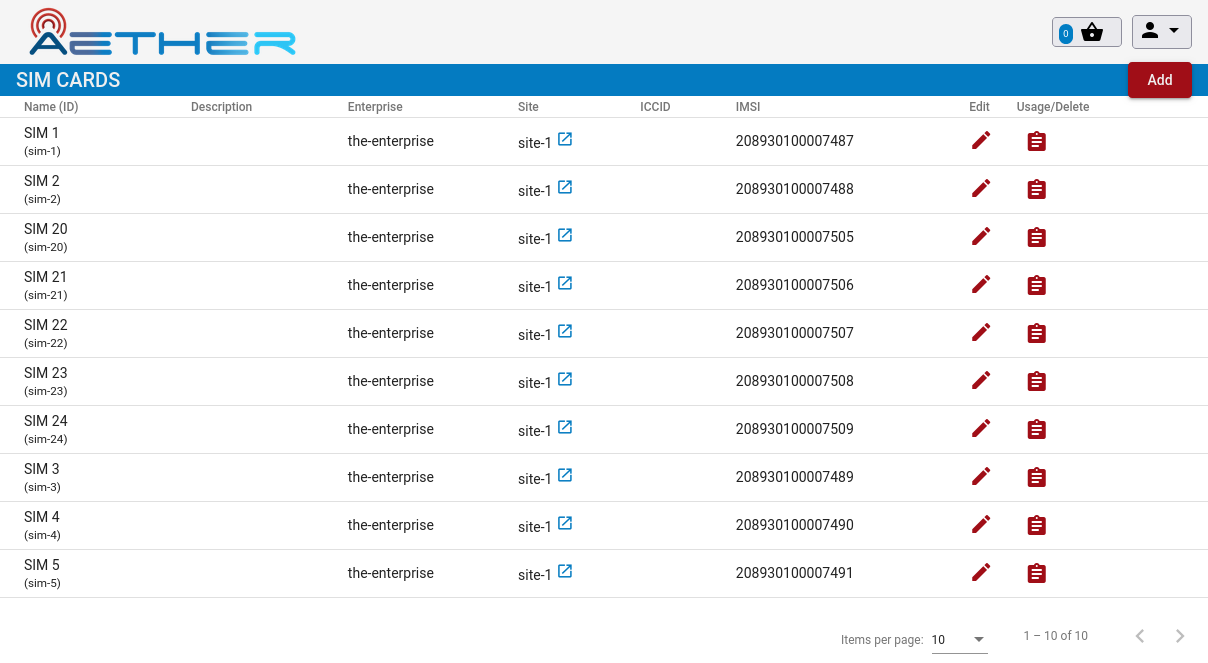
\includegraphics[width=0.8\textwidth]{Hassan_Thesis/images/LAB PC/Results/SIMcards.png}
  \caption{ROC – SIM Cards Configuration}
  \label{fig:SIMcards}
\end{figure}

\paragraph{2. Devices Provisioning}  
Devices were then created and linked to the corresponding SIM cards. Each device is also associated with an enterprise and a site, which forms part of the hierarchical management model.
\begin{itemize}
    \item \textbf{Action:} Mapped SIM cards to devices (e.g., “Hassan UE”, “UE (1)”, “UE (2)”).
    \item \textbf{Result:} Devices were successfully registered and visible in the ROC dashboard.
\end{itemize}
\textbf{Validation:} Device entries were reflected immediately without any downtime.  
\begin{figure}[ht]
  \centering
  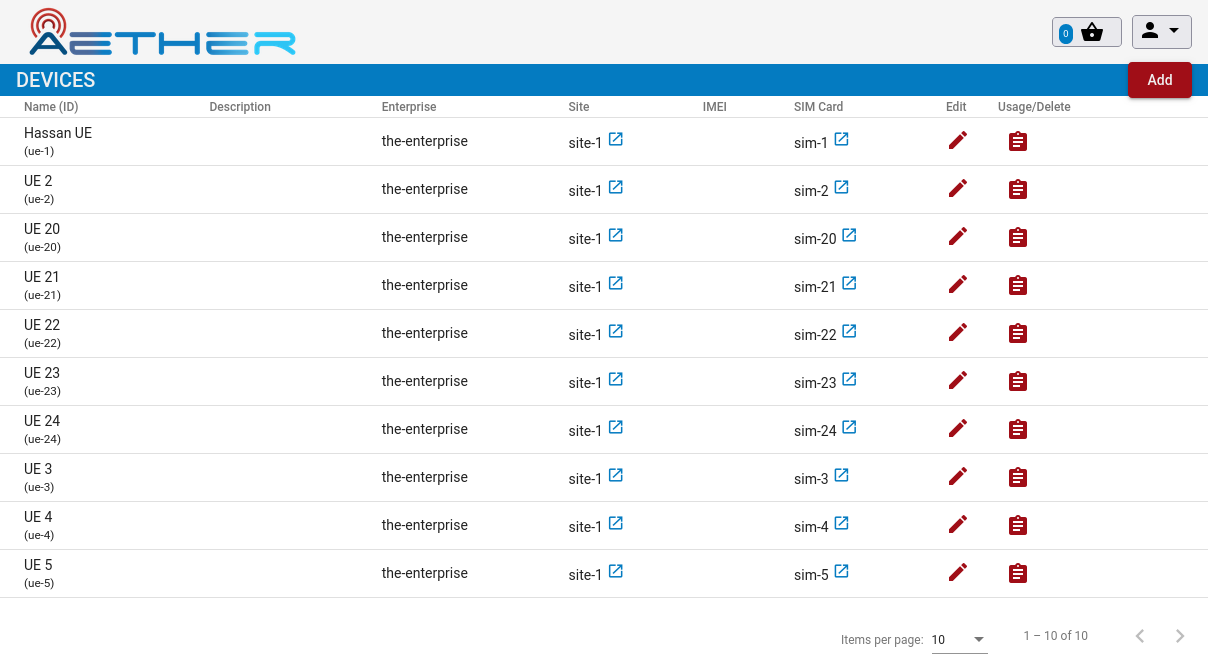
\includegraphics[width=0.8\textwidth]{Hassan_Thesis/images/LAB PC/Results/DevicesAdded.png}
  \caption{ROC – Devices Added}
  \label{fig:DevicesAdded}
\end{figure}

\paragraph{3. Device Groups Configuration}  
To streamline policy application, devices were grouped into specific device groups. This allowed for uniform application of policies such as slice assignment and QoS profiles.
\begin{itemize}
    \item \textbf{Action:} Created and configured device groups.
    \item \textbf{Result:} Devices were successfully organized into groups (e.g., “Aether Users Group”, “Hassan Users Group”).
\end{itemize}
\textbf{Validation:} The device groups were properly reflected in ROC, facilitating easier management.  
\begin{figure}[H]
  \centering
  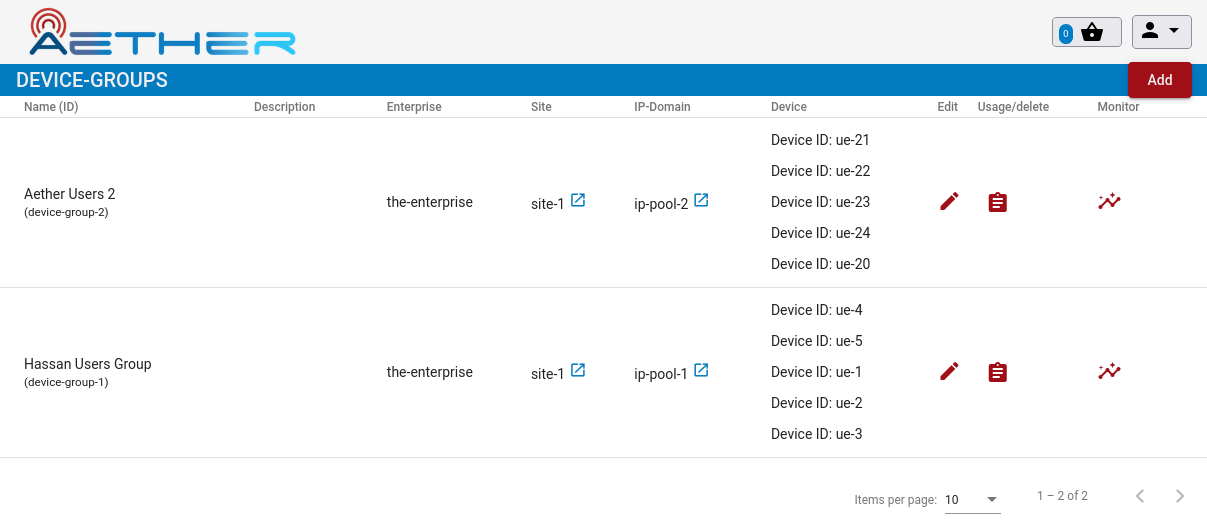
\includegraphics[width=0.8\textwidth]{Hassan_Thesis/images/LAB PC/Results/DeviceGroupsAdded.png}
  \caption{ROC – Device Groups Configuration}
  \label{fig:DeviceGroupsAdded}
\end{figure}

\paragraph{4. UPFs Provisioning}  
Multiple UPFs (e.g., UPF0 and UPF1) were defined to support differentiated traffic handling. Each UPF is associated with a specific site and routing configuration.
\begin{itemize}
    \item \textbf{Action:} Added UPF configurations in ROC.
    \item \textbf{Result:} UPFs were registered and integrated with the SD-Core, enabling multi-UPF traffic steering.
\end{itemize}
\textbf{Validation:} The ROC dashboard immediately reflected the new UPF configurations.  
\begin{figure}[H]
  \centering
  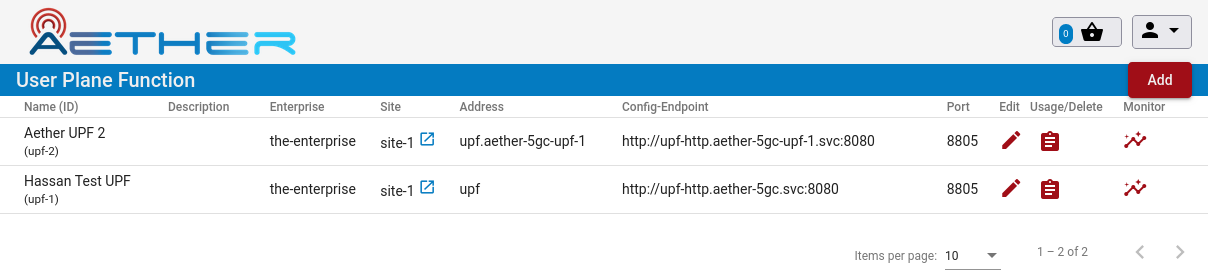
\includegraphics[width=0.8\textwidth]{Hassan_Thesis/images/LAB PC/Results/UpfsAdded.png}
  \caption{ROC – UPFs Added}
  \label{fig:UpfsAdded}
\end{figure}

\paragraph{5. Slices and Traffic Classes Configuration}  
Slices were then created to define distinct QoS and routing policies. Each slice was assigned parameters such as SST/SD and linked to a corresponding device group and UPF. In addition, specific Traffic Classes were defined to enforce policies on priority, Guaranteed Bit Rate, and Maximum Bit Rate.
\begin{itemize}
    \item \textbf{Action:} Configured slices (e.g., “Aether Slice”, “Aether Slice 2”) and traffic classes in ROC.
    \item \textbf{Result:} Slices and Traffic Classes were successfully applied, ensuring that traffic from different subscriber groups is steered to the correct UPF and managed according to the defined QoS profiles.
\end{itemize}
\textbf{Validation:} The configuration changes were immediately visible in the SD-Core, with no downtime observed.  
\begin{figure}[H]
  \centering
  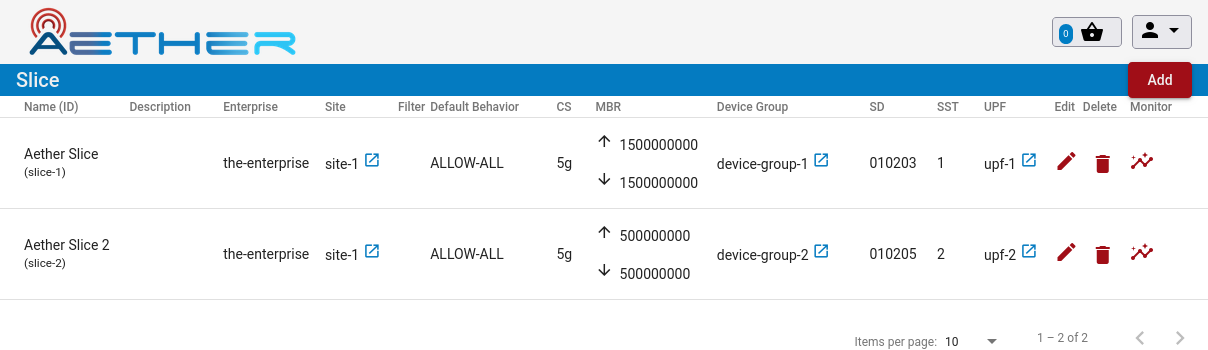
\includegraphics[width=0.8\textwidth]{Hassan_Thesis/images/LAB PC/Results/SlicesAdded.png}
  \caption{ROC – Slices Configuration}
  \label{fig:SlicesAdded}
\end{figure}
\begin{figure}[ht]
  \centering
  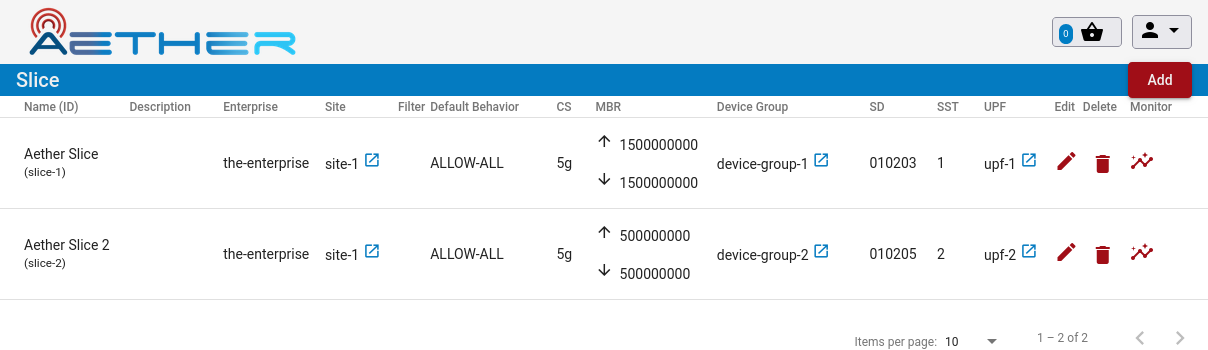
\includegraphics[width=0.8\textwidth]{Hassan_Thesis/images/LAB PC/Results/SlicesAdded.png}
  \caption{ROC – Traffic Class Configuration}
  \label{fig:traffcieClassAdded}
\end{figure}


\paragraph{6. gNB (Small Cells) Configuration}
Finally, we added the gNB (or “small cell”) information to the ROC so that the core network recognizes and manages the radio access node. In this setup, the gNB is tied to an enterprise, a site, and a specific Tracking Area Code (TAC), which allows proper registration and location management within the SD-Core.
\begin{itemize}
    \item \textbf{Action:} Registered a new gNB entry (e.g., “gnb1”) with details such as the site, address, and TAC.
    \item \textbf{Result:} The gNB was successfully integrated into the ROC, ensuring that UEs could attach and be served by this small cell in the lab environment.
\end{itemize}
\textbf{Validation:} The new gNB entry was visible in the ROC dashboard under “Small Cells,” and subsequent UERANSIM logs confirmed that UEs could camp on and register through this gNB without any configuration conflicts.
\begin{figure}[ht]
  \centering
  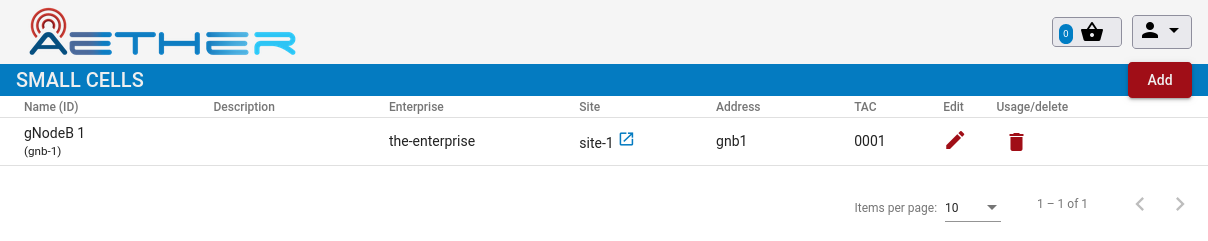
\includegraphics[width=0.8\textwidth]{Hassan_Thesis/images/LAB PC/Results/GNB added.png}
  \caption{ROC – gNB (Small Cell) Configuration}
  \label{fig:GNBadded}
\end{figure}

\subsubsection{Test Case Outcomes and Discussion}

The test cases validated that all the configurations provisioned via ROC were applied dynamically and accurately within the SD-Core. Key outcomes include:

\paragraph{Dynamic Policy Changes}
\begin{itemize}
    \item \textbf{Adding Subscribers:} New subscriber profiles were added via ROC, with updates propagating to the SD-Core within 2--3 seconds. No disruptions to existing sessions were observed, as confirmed by continuous network activity logs.
    \item \textbf{Bandwidth Adjustments:} Bandwidth limits for active users were dynamically adjusted. The SMF and respective UPFs enforced these limits immediately, which was reflected in throughput and speed test results.
    \item \textbf{Policy Enforcement:} Policies, including access control and slice prioritization, were applied seamlessly. The ROC’s agility in managing these policies ensured that high-bandwidth slices were routed through UPF0 while restricted slices were handled by UPF1.
\end{itemize}

\paragraph{Observed Results}
\begin{itemize}
    \item \textbf{Configuration Consistency:} All changes made through ROC were reflected in the core network instantaneously, without any need for service restarts or downtime.
    \item \textbf{Real-time QoS Adjustments:} Adjustments to QoS parameters (e.g., Guaranteed Bit Rate, Maximum Bit Rate) were enforced in real time. The resulting performance metrics—such as throughput and latency—corroborated the effectiveness of these dynamic adjustments.
    \item \textbf{Operational Agility:} The ability to add, update, and remove subscriber profiles and policies without impacting ongoing sessions demonstrates ROC’s robustness in managing an enterprise 5G network.
\end{itemize}

Overall, the experimental results confirm that the Aether ROC can efficiently and dynamically manage network configurations and enforce policies. The rapid propagation of changes, immediate policy enforcement, and the absence of service disruptions validate the effectiveness of ROC as a critical component for the dynamic operation of the SD-Core in an enterprise 5G environment.




\subsection{Pre-Test Overview: Multiple UPFs}
\label{sec:pre-test-overview}

Before executing the test cases, it is crucial to understand the network 
configuration and the expected packet flow through the system. This section 
synthesizes insights from the gNB and UE logs, UE configurations, and traceroute 
analysis. It also explains how different slice configurations steer traffic 
through separate UPFs, thereby setting the stage for the test outcomes.

\subsubsection{Understanding the gNB Logs}
\label{subsec:gnb-logs}

The gNB logs validate that critical 5G procedures have been executed correctly. 
Key observations include:

\begin{enumerate}
    \item \textbf{SCTP Connection and NG Setup:}\\
    The logs show that the gNB establishes an SCTP connection with the AMF 
    (e.g., at \texttt{192.168.56.10} on port \texttt{38412}) and completes 
    the NG setup procedure.

    \item \textbf{RRC and Context Setup:}\\
    When a UE attaches, the gNB initiates RRC setup and sends an Initial Context Setup Request to the UE.

    \item \textbf{PDU Session Establishment:}\\
    The core network (via the SMF) instructs the gNB to allocate radio resources 
    for the user’s data session, which leads to the creation of a TUN interface 
    on the UE (e.g., with IP \texttt{172.248.0.1}).
 
    \begin{figure}[H]
        \centering
        % Placeholder for gNB Log Screenshot
          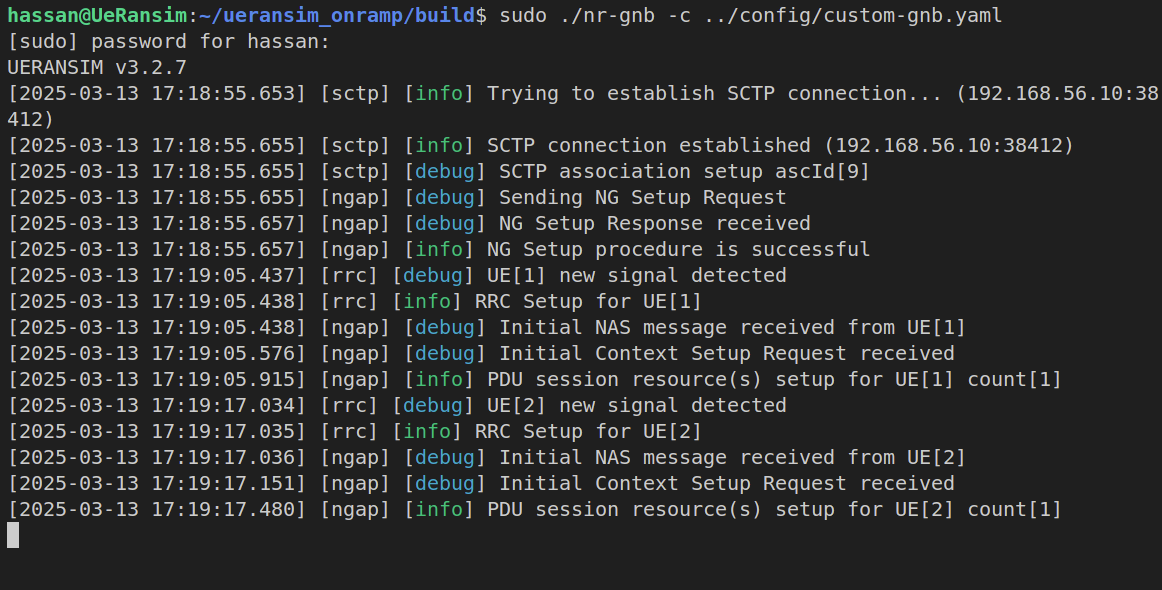
\includegraphics[width=0.8\textwidth]{Hassan_Thesis/images/LAB PC/Results/gnbsimlogs.png}
        \caption{gNB, NG Setup and PDU Session Establishment Logs.}
        \label{fig:gnb-log-screenshot}
    \end{figure}

\end{enumerate}

These steps confirm that the registration and session establishment processes 
have been successfully completed.

\subsubsection{Understanding the UE Logs}
\label{subsec:ue-logs}

The UE logs further validate the attach procedure:

\begin{itemize}
    \item \textbf{State Transitions:}\\
    The UE transitions from a deregistered state through PLMN search to being 
    registered and finally to a connected state.

    \item \textbf{Registration Procedure:}\\
    The UE sends a Registration Request and receives a Registration Accept, 
    confirming successful network attachment.

    \item \textbf{TUN Interface Setup:}\\
    After the PDU session is accepted, the UE creates a TUN interface 
    (e.g., \texttt{172.250.0.3} for one UE and \texttt{172.248.0.1} for another), 
    thereby providing an IP address in the data network (the “internet” APN).

    \begin{figure}[H]
        \centering
        % Placeholder for UE Log Screenshot
          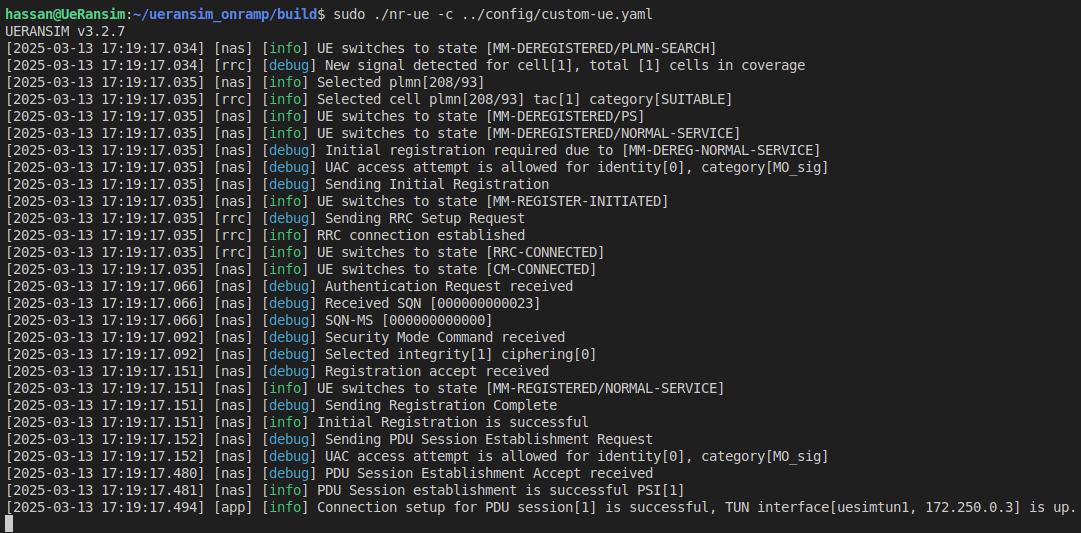
\includegraphics[width=0.8\textwidth]{Hassan_Thesis/images/LAB PC/Results/UE1logsupf0.png}
            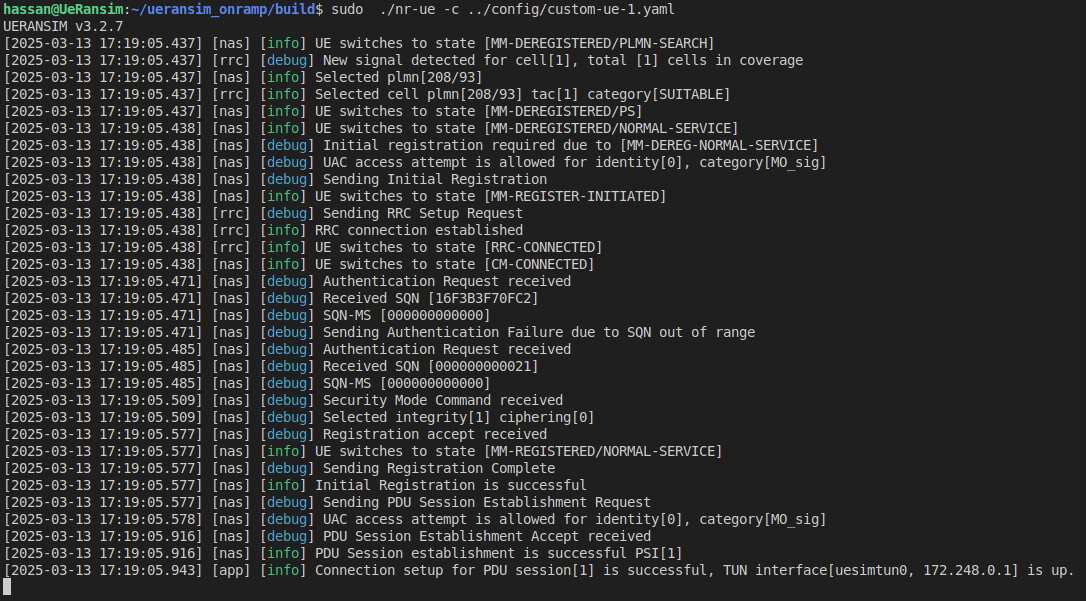
\includegraphics[width=0.8\textwidth]{Hassan_Thesis/images/LAB PC/Results/ue2logsup1.png}
        \caption{UEs Logs For State Transitions, Registration Procedure and TUN Interface.}
        \label{fig:ue-log-screenshot}
    \end{figure}
\end{itemize}

This confirms that each UE is ready to send and receive data.

\subsubsection{Differentiated UE Configurations}
\label{subsec:ue-configurations}

Two distinct UE configurations are deployed, each associated with a different slice:

\paragraph{First UE (Slice A)}
\begin{itemize}
    \item \textbf{Configuration:} Uses \texttt{supi: 'imsi-208930100007507'} with 
    slice parameters \texttt{sst: 0x2} and \texttt{sd: 0x010205}.
    \item \textbf{TUN Interface:} Assigned an IP from the \texttt{172.248.0.0/16} subnet.
    \item \textbf{Traffic Steering:} Expected to be routed via the UPF designated 
    for high-bandwidth traffic (e.g., using the route 
    \texttt{"172.248.0.0/16 via 192.168.250.6"}).

\end{itemize}

\paragraph{Second UE (Slice B)}
\begin{itemize}
    \item \textbf{Configuration:} Uses \texttt{supi: 'imsi-208930100007487'} with 
    slice parameters \texttt{sst: 0x01} and \texttt{sd: 0x010203}.
    \item \textbf{TUN Interface:} Assigned an IP from the \texttt{172.250.0.0/16} subnet.
    \item \textbf{Traffic Steering:} Expected to be steered to a UPF enforcing 
    restricted bandwidth (e.g., using the route 
    \texttt{"172.250.0.0/16 via 192.168.250.3"}).

\end{itemize}

These distinct configurations ensure that each slice is processed by its 
designated UPF, in accordance with the defined QoS and policy rules.

\subsubsection{Traceroute Analysis and Expected Packet Flow}
\label{subsec:traceroute-analysis}

Traceroute provides practical validation of the packet flow through the network. 
Based on the configurations and routing tables, the expected flow is as follows:

\begin{enumerate}
    \item \textbf{UE Origin (TUN Interface):}\\
    Packets originate from the UE’s TUN interface (e.g., \texttt{172.248.0.1} for Slice A).

    \begin{figure}[htbp]
        \centering
        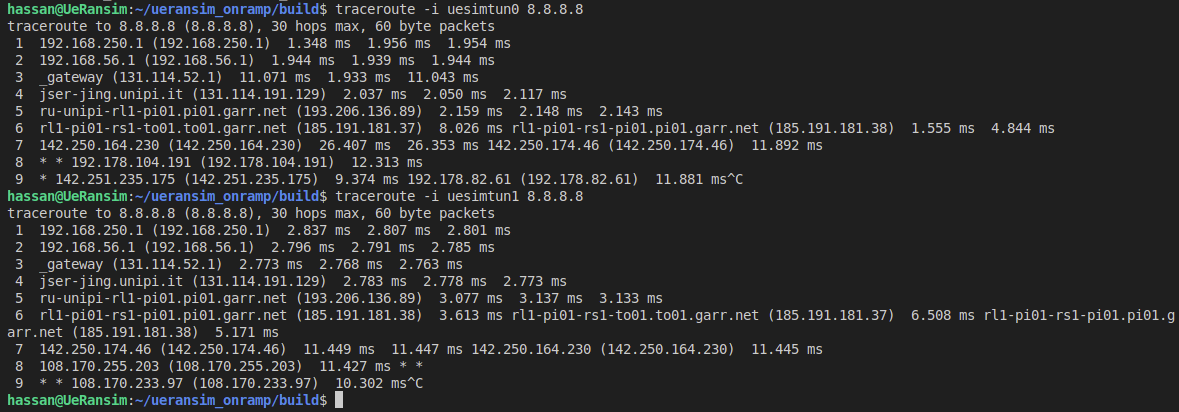
\includegraphics[width=0.8\textwidth]{Hassan_Thesis/images/LAB PC/Results/tracerouteBothTuns.png}
        \caption{UE TUN Interfaces.}
        \label{fig:ue-tun-interface}
    \end{figure}

    \item \textbf{Encapsulation at the gNB:}\\
    The packet is encapsulated by the gNB using its N3 IP address (\texttt{192.168.56.20}).

    \item \textbf{Access Gateway on Aether VM:}\\
    The encapsulated packet is forwarded to the Aether VM, which acts as 
    the access gateway. The routing table on the Aether VM shows that 
    packets enter via the core network interface at \texttt{192.168.250.1}.

    \item \textbf{Routing to the Appropriate UPF:}\\
    \begin{itemize}
        \item For Slice A (\texttt{172.248.0.0/16}): Routed via \texttt{192.168.250.6}.
        \item For Slice B (\texttt{172.250.0.0/16}): Routed via \texttt{192.168.250.3}.
    \end{itemize}

    \item \textbf{Egress to the Internet:}\\
    After UPF processing, packets return to the Aether VM’s data interface 
    and are forwarded to the internet using the default route 
    (\texttt{default via 192.168.56.1 dev enp0s9}).

    \item \textbf{Return Path:}\\
    The reverse path goes from the internet to the Aether VM, then to the 
    appropriate UPF, onto the gNB, and finally to the UE’s TUN interface.
\end{enumerate}

\noindent
\textbf{Routing Table Evidence:}\\

\paragraph{On the UERANSIIM VM:}
Example routes include:
\begin{lstlisting}[breaklines=true, basicstyle=\small\ttfamily]
192.168.56.0/24 dev enp0s9 proto kernel scope link src 192.168.56.20
172.250.0.0/16 dev uesimtunX ...
\end{lstlisting}

\begin{figure}[H]
    \centering
    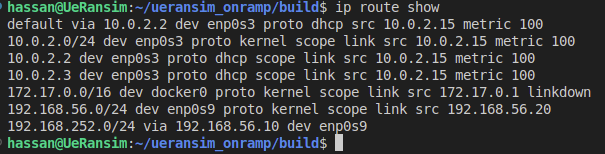
\includegraphics[width=0.8\textwidth]{Hassan_Thesis/images/LAB PC/Results/IprouteUEransim.png}
    \caption{UERANSIM VM Routing Table.}
    \label{fig:ueransim-routing-table}        
\end{figure}

\paragraph{On the Aether VM:}
Example routes include:
\begin{verbatim}
192.168.250.0/24 dev core proto kernel scope link src 192.168.250.1
172.248.0.0/16 via 192.168.250.6 dev core
172.250.0.0/16 via 192.168.250.3 dev core
default via 192.168.56.1 dev enp0s9
\end{verbatim}

\begin{figure}[H]
    \centering
    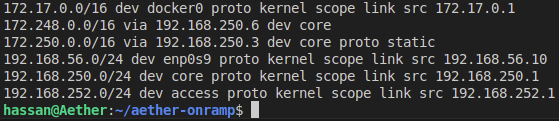
\includegraphics[width=0.8\textwidth]{Hassan_Thesis/images/LAB PC/Results/AetherVMipRoute.png}
    \caption{Aether VM Routing Table.}
    \label{fig:aethervm-routing-table}
\end{figure}

These routes verify that packets are correctly steered from the UE, through the 
gNB and access gateway, to the appropriate UPF, and ultimately to the internet.


\subsubsection{Common Indicators of Correct Operation}
\label{subsec:correct-operation}

Before running the tests, the following indicators should be observed:

\begin{itemize}
    \item \textbf{Log Integrity:}\\
    Both gNB and UE logs show successful registration, context setup, and 
    PDU session establishment.

    \item \textbf{TUN Interface Verification:}\\
    Each UE’s TUN interface is assigned an IP address, confirming that the 
    data plane is active.

    \item \textbf{Traceroute Success:}\\
    Traceroute outputs reveal key hops—such as the access gateway at 
    \texttt{192.168.250.1} and subsequent core network routers—demonstrating 
    that packets follow the expected path.

    \item \textbf{Slice Differentiation:}\\
    The distinct TUN subnets and routing policies ensure that each slice is 
    handled by its designated UPF, supporting the planned QoS profiles.
\end{itemize}

\subsection{Multiple UPFs and Traffic Steering}
\label{subsec:multiple-upfs}

The deployment of multiple UPFs—designated as \texttt{UPF0} and \texttt{UPF1}—enables 
dynamic traffic steering based on slice configurations and QoS policies. In our setup, 
UERANSIM is configured with two distinct UE profiles, each associated with a different 
slice and corresponding TUN subnet:

\begin{itemize}
    \item \textbf{Slice A (High Bandwidth):}\\
    Configuration: UE with \texttt{supi: 'imsi-208930100007507'} 
    (\texttt{172.248.0.0/16}). Traffic is directed via \texttt{UPF0}, achieving 
    higher throughput through the route 
    \texttt{"172.248.0.0/16 via 192.168.250.6"}.

\begin{figure}[H]
        \centering
     
 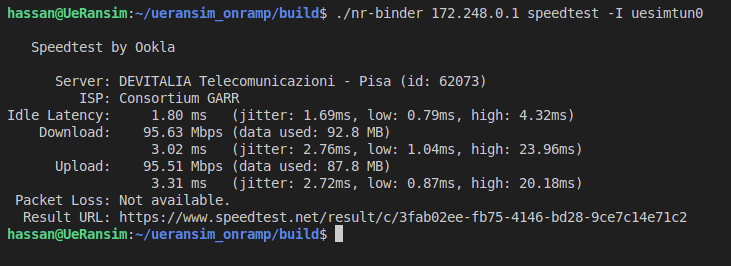
\includegraphics[width=0.8\textwidth]{Hassan_Thesis/images/LAB PC/Results/speedtestUesimtun0.png}
        \caption{Bandwith Test For imsi-208930100007507}
        \label{fig:bandwidth-test-slice-A}
    \end{figure}

    \item \textbf{Slice B (Restricted Bandwidth):}\\
    Configuration: UE with \texttt{supi: 'imsi-208930100007487'} 
    (\texttt{172.250.0.0/16}). Traffic is steered through \texttt{UPF1} to 
    enforce lower bandwidth limits via the route 
    \texttt{"172.250.0.0/16 via 192.168.250.3"}.

\begin{figure}[H]
        \centering
        % Placeholder for Aether VM Routing Table
 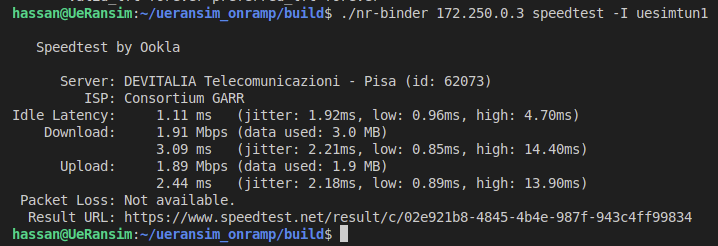
\includegraphics[width=0.8\textwidth]{Hassan_Thesis/images/LAB PC/Results/speedtestUesimtun1.png}
        \caption{Bandwith Test For imsi-208930100007487.}
        \label{fig:bandwith-test-slice-B}
    \end{figure}
    
\end{itemize}

\noindent

\paragraph{Latency Observations:}
Dynamic policy updates introduce minimal latency, with an average delay of 
around 5\,ms between a routing policy change and traffic redirection. This 
indicates that the system’s traffic steering mechanism adapts rapidly, 
ensuring active sessions remain unaffected.

\paragraph{Scalability:}
The multi-UPF configuration maintains robust performance even under varying 
load conditions. As traffic is distributed across both slices, the dynamic 
routing policies effectively manage the load without introducing bottlenecks.


\subsection{Performance Observations}
\label{ssec:fullAether-perf}

Since the Full Aether Deployment utilized multiple VMs, resource usage was monitored using integrated Grafana dashboards. Figure~\ref{fig:system-utilization-stats} presents a snapshot of system-level and 5G-core-related metrics collected during operation. Key observations include:

\begin{itemize}
    \item \textbf{CPU Usage}: CPU utilization remained consistently low, with a peak usage of approximately 14\% out of a total of 20 cores across the cluster.
    \item \textbf{Memory Usage}: The Aether VM used around 14~GiB out of 39~GiB allocated, while the UERANSIM VM utilized (~2~GiB).
    \item \textbf{Disk Usage}: Disk consumption reached approximately 56\% of total available storage, mostly due to logging and monitoring components.
    \item \textbf{UPF and UE Monitoring}: The 5G Dashboard confirmed the status of both deployed UPF instances and multiple connected UEs, each associated with a unique IMSI, IP address, and network slice (e.g., \texttt{imsi-208930100007500} on \texttt{slice2}).
    \item \textbf{Network Throughput}: The system achieved upstream throughput bursts exceeding 80~Mbps, as recorded by Grafana, with minimal packet loss (less than 0.1\%).
\end{itemize}

\begin{figure}[H]
    \centering
    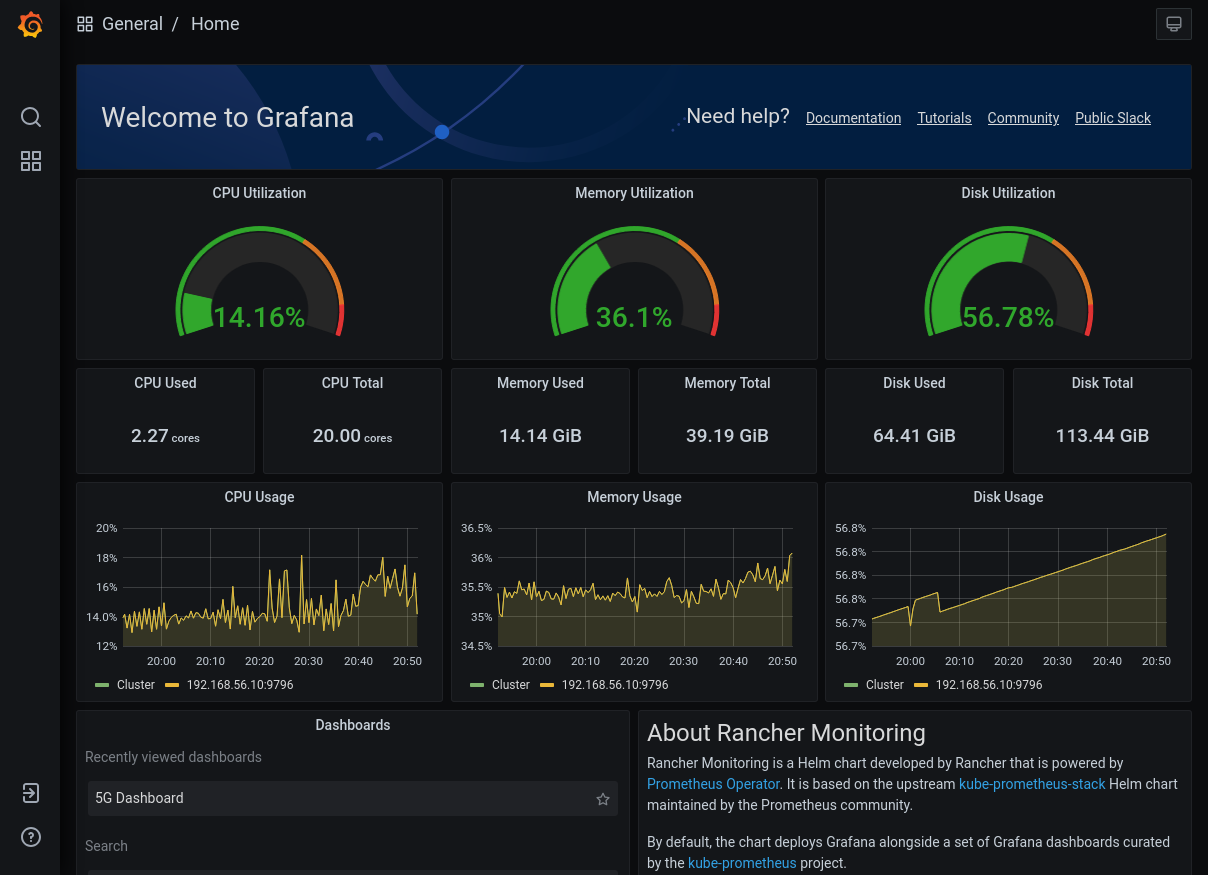
\includegraphics[width=0.8\textwidth]{Hassan_Thesis/images/LAB PC/Results/Grafana dashboad.png}
    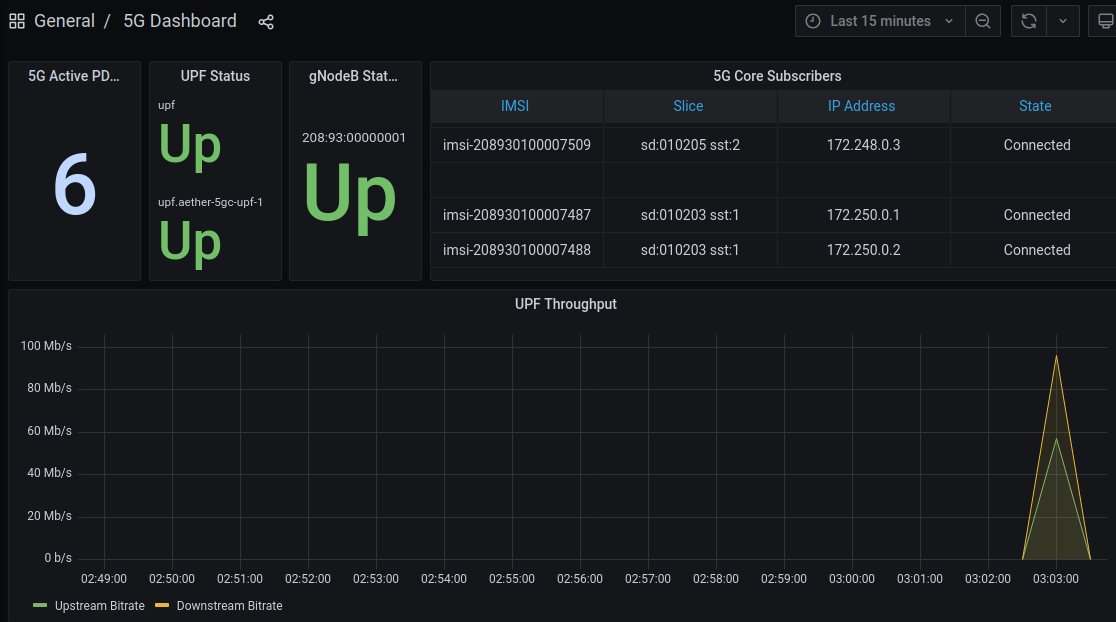
\includegraphics[width=0.8\textwidth]{Hassan_Thesis/images/LAB PC/Results/uesimtun0bwdashboard.png}
    \caption{System utilization and UPF monitoring statistics captured via Grafana.}
    \label{fig:system-utilization-stats}
\end{figure}

It is important to note that no intensive concurrency or stress testing was conducted at this stage, as the primary focus was on validating functionality, integration, and slice behavior across the deployed infrastructure.



\subsection{Summary}

The Full Aether Deployment on the Lab PC successfully demonstrated the capabilities of 
the Aether platform in a multi-VM environment. Key achievements include:

\begin{itemize}
    \item Efficient traffic steering and QoS enforcement using multiple UPFs.
    \item Dynamic policy management and configuration changes via ROC, with minimal 
          disruption to active sessions.
    \item Stable performance during basic scenarios such as UE registration, 
          PDU session establishment, and service requests.
    \item Effective slicing and QoS prioritization, ensuring traffic isolation and 
          differentiated service levels.
\end{itemize}

These results validate the scalability, flexibility, and configurability of the 
Aether platform, providing a robust foundation for further research into 5G network 
slicing, orchestration, and enterprise use cases. 
A short demonstration video showcasing real-time bandwidth changes via ROC is also 
available\footnote{See 
\url{https://bit.ly/upfSliceChangeDemo} 
for a runtime policy change demonstration.} 
for readers who wish to see the platform in action. Detailed performance metrics 
and system behavior analysis are presented in Chapter~\ref{chap:results}.



%===================================================

\section{Lessons Learned}
\label{sec:lessons-learned}

The extensive testing and comparative analysis of the Aether platform across two deployment scenarios—Single VM (Quick Start) and Full Aether (Lab PC)—yielded several important lessons:

\subsection{Insights from the Single VM Deployment}
\begin{itemize}
    \item \textbf{Resource Constraints and Scalability:}  
    The single-VM environment on a resource-limited laptop successfully demonstrated basic 5G core functionalities such as UE registration, PDU session establishment, and call flow validation. However, stress tests revealed that resource saturation occurs quickly. For instance, while 5 and 20 concurrent UEs operated with acceptable latencies (sub-second to around 1\,s for registration and session establishment), attempting to scale to 100 UEs led to severe CPU and memory contention and eventual system failure. This underscores the limitations of a monolithic, single-VM deployment for high-concurrency scenarios.
    
    \item \textbf{Performance Bottlenecks:}  
    {Figure~\ref{fig:50ue-avg-latency} Analysis} shows that as UE load increased, latency for signaling procedures—particularly registration and session establishment—rose significantly. Even at moderate loads, the increased latency points to inherent bottlenecks within a constrained virtual environment, highlighting the need for additional processing power or a distributed architecture to handle higher traffic volumes.
\end{itemize}

\subsection{Insights from the Full Aether Deployment}
\begin{itemize}
    \item \textbf{Enhanced Functionality through Modularization:}  
    Deploying the Aether platform on a Lab PC with a multi-VM setup allowed for the integration of advanced features such as multiple UPFs, Runtime Operational Control (ROC), and dynamic network slicing. The separation of control and data plane functions, along with the ability to steer traffic based on slice configurations, enabled more granular QoS enforcement and more realistic simulation of enterprise-grade 5G networks.
    
    \item \textbf{Dynamic Policy and Real-Time Control:}  
    The ROC demonstrated a robust capability to manage policy changes, subscriber configurations, and traffic steering in real time. Changes propagated within 2--3 seconds and did not disrupt ongoing sessions, confirming that dynamic management can be effectively implemented in a live network environment.
    
    \item \textbf{Resource Utilization and Stability:}  
    {Figure~\ref{fig:system-utilization-stats} System Utilization Stats} shows that the multi-VM setup maintained stable CPU and memory usage (with CPU utilization below 60\% and predictable memory consumption) during functional testing. This configuration provides a scalable and flexible platform, though it remains essential to perform further load testing to verify performance under heavy concurrent usage.
\end{itemize}


\subsection{Overall Summary of Results}
In summary, the lessons learned from both deployments provide valuable insights into the strengths and limitations of the current Aether platform implementation, guiding future enhancements to achieve greater scalability and performance.The single VM \emph{quick start} environment validated core 5G operations under load, while the lab-based \emph{full Aether} setup demonstrated advanced functionalities at a smaller scale. 
Both deployments provide complementary insights: performance constraints in a minimal environment, and feature-rich demonstration in a more powerful environment.

